\documentclass[11pt,a4paper]{article}
\usepackage[margin=2.2cm]{geometry}
\usepackage{amsmath,amssymb}
\usepackage{graphicx}
\usepackage{booktabs}
\usepackage{siunitx}
\usepackage[colorlinks=true,linkcolor=blue,citecolor=blue,urlcolor=blue]{hyperref}
\graphicspath{{../plots/}}
\sisetup{separate-uncertainty=true}

\newcommand{\MV}{M_V}
\newcommand{\feh}{[\mathrm{Fe/H}]}
\newcommand{\dhel}{d}
\newcommand{\avg}[1]{\left\langle #1 \right\rangle_t}

\title{Completeness of the Milky Way globular-cluster catalogue\\from the phases of cluster orbits}
\author{Draft prepared with Claude Code for V.~Belokurov}
\date{\today}

\begin{document}
\maketitle

\begin{abstract}
We estimate how the completeness of the Milky Way globular-cluster (GC) catalogue depends on
absolute magnitude and heliocentric distance, using the 165 GCs with full six-dimensional phase-space
data. The estimator conditions on each cluster's own orbit: if clusters are phase-mixed, the
present position of a detected cluster samples its orbit with probability proportional to the
completeness $C$ at that point. Maximising the resulting likelihood needs no model of the
intrinsic GC density. On mock catalogues with known selection it recovers completeness without bias
and with calibrated intervals (recovered/true $=0.97$--$0.99$, 68\% coverage $0.67$--$0.71$). A
fixed-target orbit-superposition estimator in the spirit of Khoperskov et al.\ (2025) is biased high
by $\approx 25\%$ on the same mocks. Applied to the data with $C$ a function of
extinction-free apparent magnitude $V$, completeness falls from 1 at $V<6$ (assumed) to $0.14$ at
$V>11$. Weighting each cluster by the inverse of its orbit-averaged completeness turns 165 observed
GCs into $483$ ($68\%$: $335$--$765$). Adding extinction along every orbit from 3D dust maps
(DECaPS, Bayestar19, Marshall, with SFD beyond their reach) improves the fit by
$\Delta\mathrm{AIC}\approx 8$ and \emph{lowers} the corrected total: without extinction the fitted
$C(V)$ absorbs the dust losses of the inner Galaxy and applies them in every direction, inflating the
weights of distant halo clusters. A continuous $C(V)$ whose faint tail keeps falling fits better
still and removes a factor-of-two undercount of faint clusters in mocks. Letting completeness differ
between the inner Galaxy ($|l|<30^\circ$, $|b|<15^\circ$) and the rest of the sky recovers such an effect
in mocks; on the data it is preferred without extinction ($\Delta\mathrm{AIC}=-4.2$) but not once the
maps are included, where two- or three-region variants change the total by $-12$ to $+12\%$. Our final estimate (continuous
$C(V)$, maps, own-orbit weights) is $N_{\rm GC}\approx430^{+215}_{-125}$ (68\%, sampling and quantified
systematics), of which about 210 ($125$--$325$) are fainter than $\MV=-6.5$; three $1/V_{\max}$-type weightings over orbit populations give 393--432 (faint 177--208). In
mocks matched to the observed sample the bootstrap intervals are calibrated (68\% coverage
0.63--0.79) and no weighting is significantly better than another. The data favour at most a mild
increase of orbit size towards fainter clusters. The dominant uncertainties are systematic: the
extinction treatment (a factor of 1.7), the assumption that the brightest clusters are complete, and
the Galactic potential.
\end{abstract}

%======================================================================
\section{How the method works, in brief}
\label{sec:brief}

\paragraph{The idea.} If a cluster is caught in only a small fraction of the places its orbit takes
it, it must have siblings that sit in the uncaught parts of their orbits right now. We count them.

\paragraph{Ingredients.} For each catalogued cluster we integrate its orbit for 5 Gyr and record it at
500 moments. At each moment we compute how bright it would look from the Sun,
$V = \MV + 5\log_{10}(d/10\,\mathrm{pc}) + A_V$. This gives the cluster's \emph{time fractions}: how
long it spends looking like each value of $V$. The catalogue adds one fact per cluster, the $V$ it
has today.

\paragraph{Logic.} If every cluster were detected, today would be a random moment of each orbit, and
clusters would be caught at each $V$ in proportion to the time they spend there. If clusters
looking faint are harder to detect, we catch them preferentially in their bright phases. The mismatch
between where clusters are caught and where they spend their time measures how detection falls
with $V$.

\paragraph{A worked example.} Take two brightness bins, bright (B) and faint (F), and one unknown,
$r = C_F/C_B$: how much less often a cluster is detected while it looks faint than while it looks
bright ($r=1$: no selection; $r=0$: never detected when faint). Three clusters:

\begin{center}
\small
\begin{tabular}{lccc}
\toprule
Cluster & Time looking bright & Time looking faint & Seen today \\
\midrule
1 & 50\% & 50\% & B \\
2 & 20\% & 80\% & B \\
3 & 10\% & 90\% & F \\
\bottomrule
\end{tabular}
\end{center}

The chance of catching a cluster in a bin is its time there times the detection probability there,
divided by the same sum over both bins. For cluster 1, caught bright, this is
$0.5\,C_B/(0.5\,C_B + 0.5\,C_F) = 1/(1+r)$: $C_B$ cancels, so the positions measure only the ratio
$r$. For clusters 2 and 3 the chances are $1/(1+4r)$ and $9r/(1+9r)$. The clusters are independent, so
the probability of seeing all three where they are is the product, the likelihood
\begin{equation}
L(r) = \frac{1}{1+r}\times\frac{1}{1+4r}\times\frac{9r}{1+9r}.
\end{equation}
It is $0.090$ at $r=1$, $0.277$ at $r=0.25$, $0.314$ at $r=0.13$ and $0.246$ at $r=0.05$. Its maximum
is at $r\approx0.13$. Clusters 1 and 2 spend most of their time faint but are caught bright, which
rules out weak selection. Cluster 3 is caught faint, which rules out $r\approx0$. The fit is the
compromise.

\paragraph{The anchor.} The likelihood fixes only ratios. Assuming bright-looking clusters are all
detected, $C_B=1$, gives $C_F = 0.13$. This is set once, for the whole function, not per cluster.

\paragraph{The weights.} Each cluster's overall detection chance $q$ is $C$ averaged over its own time
fractions: $q_1 = 0.5 + 0.5\times0.13 = 0.565$, $q_2 = 0.2 + 0.8\times0.13 = 0.304$,
$q_3 = 0.1 + 0.9\times0.13 = 0.217$. Each stands for $1/q$ clusters: $1.8 + 3.3 + 4.6 \approx 9.7$
clusters from the 3 observed.

\paragraph{No luminosity function is needed.} We never compare counts at different luminosities. Each
cluster is compared only with its own orbit, and the probability of catching it at a given phase
depends on its orbit, its own (measured) $\MV$ and $C$, not on how common clusters of its
luminosity are. In a toy population where half of each orbit looks bright and half faint, the number
of clusters in a luminosity group changes how many we see, not the near/far split of those we see.
The corrected histogram of $\MV$ is then an \emph{output}: the luminosity function. The price is the
assumption that replaces it: clusters are at random phases of their orbits today (phase mixing),
whatever their luminosity.

\paragraph{The real analysis} is the same procedure with all 165 clusters, 8 bins in $V$ (7 unknown
ratios, Eq.~\ref{eq:phaselike}) and the likelihood maximised numerically. Two refinements
(Sec.~\ref{sec:vmax}) handle faint clusters. A continuous $C(V)$ keeps falling beyond the faintest
detection. And in the $1/V_{\max}$ form, a faint cluster's detection chance is averaged over the
orbits of bright clusters, which are visible almost anywhere, rather than over its own orbit alone.
This counts faint clusters on orbits where none has been seen, on the assumption that faint and
bright clusters share one orbit distribution. On mocks matched to the observed sample, neither form
is reliably better (Sec.~\ref{sec:faint}), and we quote the simpler own-orbit form as the headline.
Two further ingredients matter: extinction along each orbit (Secs.~\ref{sec:ext}, \ref{sec:nodustbias})
and, as a check, completeness that depends on direction (Sec.~\ref{sec:region}).

%======================================================================
\section{Data}
\label{sec:data}

We use the 165 confirmed GCs with full phase-space data (positions, distances, proper motions,
line-of-sight velocities and their errors) from the PI's compilation of Vasiliev \& Baumgardt (2021)
astrometry. Absolute magnitudes come from the Baumgardt combined table\footnote{Downloaded
2026-10-09 from \url{https://people.smp.uq.edu.au/HolgerBaumgardt/globular/combined_table.txt}.} as
$\MV = 4.83 - 2.5\log_{10}(M_{\rm dyn}/\Upsilon_V)$, with $M_{\rm dyn}$ the dynamical mass and
$\Upsilon_V$ the $V$-band mass-to-light ratio. Two confirmed clusters without 6D data are excluded.
Progenitor labels (in-situ: main bulge and main disc, 61 GCs; accreted: Gaia-Enceladus, Sequoia,
Helmi streams, high-energy group and Sagittarius, 64 GCs) come from the catalogue column
\texttt{PROG\_MA}; we have not verified their provenance (they appear to follow Massari et al.\ 2019).

Positions and velocities are transformed to the Galactocentric frame with the astropy v4.0 solar
parameters ($R_0 = 8.122$ kpc, $z_\odot = 20.8$ pc, $\boldsymbol v_\odot = (12.9, 245.6, 7.78)$
km\,s$^{-1}$; Astropy Collaboration 2022). Orbits are integrated with AGAMA (Vasiliev 2019) in a
static axisymmetric potential (Miyamoto--Nagai disc, $6.8\times10^{10}\,M_\odot$, $a=3.0$, $b=0.28$
kpc; two Dehnen spheroids, $5\times10^{9}\,M_\odot$ at $1.0$ kpc and $1.71\times10^{9}\,M_\odot$ at
$0.07$ kpc; NFW halo, $5.4\times10^{11}\,M_\odot$, $r_s = 15.62$ kpc), forward for 5 Gyr from the
present and sampled at 500 equal time steps. Energy is conserved to $2\times10^{-6}$. No observed
cluster and no orbit sample lies beyond 150 kpc.

%======================================================================
\section{Method}
\label{sec:method}

\subsection{Per-cluster phase likelihood}

Let cluster $i$ move on a known orbit, sampled at times $t$, with heliocentric distance
$\dhel_i(t)$. If the population is phase-mixed in a static potential, the present phase of an
undetected cluster is uniform in $t$. Detection with probability $C$ tilts that distribution, so the
present phase of a \emph{detected} cluster, conditional on its orbit, has density proportional to
$C$ at that phase. The log-likelihood of the observed present positions is
\begin{equation}
\ln \mathcal{L} = \sum_i \Big[\ln C(M_{V,i}, \dhel_{i,\rm now}) - \ln \avg{C(M_{V,i},\dhel_i(t))}\Big].
\label{eq:phaselike}
\end{equation}
Two properties make Eq.~(\ref{eq:phaselike}) useful. First, no model of the intrinsic GC density
enters. Second, conditioning on each detected orbit removes the dependence on which orbits happen to
be in the catalogue. The overall scale of $C$ cancels, so the data constrain $C$ only up to one
constant, and only over the range of $\dhel$ (or $V$) that the observed orbits span.

We take $C$ piecewise constant in bins, write $\theta_k = \ln(C_k/C_0)$ with the reference bin
$k=0$ fixed, and maximise Eq.~(\ref{eq:phaselike}) with L-BFGS-B ($-8 \le \theta_k \le 4$). The
likelihood is concave in $\theta$. Intervals are 68\% profile-likelihood intervals
($2\Delta\ln\mathcal{L}=1$). The last bin is open-ended.

\subsection{Two parameterisations of $C$}

\paragraph{$C(\MV,\dhel)$ per luminosity class.} We split the sample into three equal-count $\MV$
classes ($\approx 55$ GCs each) and, within each, into equal-count distance bins of at least 15 GCs
(three bins of 18--19 GCs). Bins are chosen once on the observed sample and then frozen. Each class
yields $C(\dhel)/C(\text{nearest bin})$; the classes are not linked to one another.

\paragraph{$C(V)$.} To link the classes we assume completeness depends on apparent magnitude only,
$C = C(V)$ with $V = \MV + 5\log_{10}(\dhel/10\,\mathrm{pc})$. This is a special case of
$C(\MV,\dhel)$: a faint cluster nearby and a bright cluster farther away with the same $V$ share
the same completeness. All 165 clusters then enter one fit, with $V_i(t)$ varying along each orbit.
We use eight equal-count bins in observed $V$ (20--21 GCs each) and fix the brightest bin
($V<6.0$) as complete, $C_0 = 1$. This single anchor makes $C$ absolute at all $\MV$. $V$ excludes
extinction; Sec.~\ref{sec:ext} tests one extinction model.

\subsection{Corrected counts}

Each observed cluster receives the weight $w_i = 1/q_i$, with $q_i = \avg{C(V_i(t))}$ its
orbit-averaged completeness. Corrected distributions are weighted histograms. This is the
Horvitz--Thompson (1952) inverse-inclusion-probability estimator with the inclusion probability
averaged over orbital phase. It corrects for incompleteness along the orbits of observed clusters; it
cannot add clusters on orbit families that are never detectable. Uncertainties on corrected counts
come from a cluster bootstrap (200 replicates): each replicate resamples clusters, refits $C$ on the
fixed bins, and sums the refitted weights of the resampled clusters.

\subsection{Symmetry tests}

If the model holds, the present position of each cluster is a draw from its orbit's $C$-weighted
phase distribution. For three statistics --- $z$, $y$ (the Galactic-longitude side) and the
azimuth from the Sun's direction $|\phi'|$ --- we compute each cluster's randomised probability
integral transform (PIT) against that distribution, pool the 165 values, and form a
Kolmogorov--Smirnov statistic. The $p$-value comes from 500 null simulations that redraw present
phases from the fitted $C$ and refit $C$ in every simulation, with a $+1$ correction.

\subsection{Comparison estimator: orbit superposition with a fixed target}

Following Khoperskov et al.\ (2025), we also fit non-negative orbit weights so that the
time-averaged occupancy of the observed orbits on an $(R,|z|)$ grid reproduces a fixed target
density (spherical broken power law with inner slope 2, outer slope 4, $r_b = 5$ kpc, $r_c = 0.3$
kpc; and variants), and take $C = N_{\rm obs}/N_{\rm corr}$ in each distance bin. Unlike
Eq.~(\ref{eq:phaselike}), this estimator depends on the assumed target density.

%======================================================================
\section{Validation on mock catalogues}
\label{sec:mocks}

Mock populations are drawn from an isotropic quasi-spherical distribution function in the same
potential, with a broken-power-law density (inner slope 2, outer slope 4, $r_b = 5$ kpc,
$r_c = 0.3$ kpc), 250 GCs per realisation and a Gaussian luminosity function
$\MV \sim \mathcal{N}(-7.4, 1.2)$. Each mock cluster sits at a uniformly random phase of its orbit
and is detected with probability $C_{\rm true} = \{1+\exp[(\MV - (V_{\rm lim} - {\rm DM}))/0.5]\}^{-1}$,
$V_{\rm lim} = 8$, so $C_{\rm true}$ is a function of $V$. Scenarios B--D break the assumptions:
B multiplies $C$ by a latitude term $1 - 0.7\,e^{-|b|/5^\circ}$; C adds a non-phase-mixed clump of
15 Sagittarius-like clusters; D makes $C$ depend on $\MV$ and $\dhel$ but not through $V$ alone. Each
estimator is compared with its own correct truth: for the phase likelihood, the value it converges to
for an infinite sample; for the target estimator, the true detected-to-intrinsic ratio per bin.

\begin{table}[h]
\centering
\caption{Mock recovery of relative completeness $C(\dhel)/C(\text{nearest bin})$ per luminosity class
(100 realisations per scenario). Ratios are recovered/true, median and 16--84\% range; coverage is
the fraction of nominal 68\% intervals containing the truth.}
\label{tab:mock_classes}
\small\setlength{\tabcolsep}{4pt}
\begin{tabular}{lccc}
\toprule
Estimator & A: assumptions hold & B: latitude-dependent $C$ & C: Sgr-like clump \\
\midrule
Phase likelihood & $0.99$ ($0.68$--$1.41$); cov.\ $0.67$ & $0.98$ ($0.71$--$1.52$); $0.71$ & $0.97$ ($0.68$--$1.34$); $0.71$ \\
Target, plain ratio & $1.29$ ($0.88$--$1.85$); $0.48$ & $1.30$; $0.54$ & $1.39$; $0.45$ \\
Target, bias-reduced & $1.23$ ($0.84$--$1.77$); $0.50$ & $1.22$; $0.58$ & $1.32$; $0.47$ \\
\bottomrule
\end{tabular}
\end{table}

\begin{table}[h]
\centering
\caption{Mock validation of $C(V)$ and the corrected counts (100 realisations per scenario).}
\label{tab:mock_cv}
\small\setlength{\tabcolsep}{4pt}
\begin{tabular}{lcccc}
\toprule
 & A: $C(V)$ true & B: latitude & C: Sgr clump & D: not $C(V)$ \\
\midrule
$C(V)$ shape, recovered/true & $0.92$ & $1.08$ & $1.01$ & $1.08$ \\
\quad 68\% coverage & $0.69$ & $0.68$ & $0.68$ & $0.67$ \\
Corrected total / true & $0.80$ ($0.60$--$1.07$) & $0.56$ & $0.71$ & $0.87$ \\
Faint ($\MV>-6.5$): observed / true & $0.15$ & $0.12$ & $0.15$ & $0.64$ \\
Faint: corrected / true & $0.44$ & $0.27$ & $0.42$ & $0.73$ \\
\bottomrule
\end{tabular}
\end{table}

Tables~\ref{tab:mock_classes} and \ref{tab:mock_cv} and Figs.~\ref{fig:mock_classes} and
\ref{fig:mock_cv} summarise the tests. The phase likelihood recovers completeness without bias and
with calibrated intervals in every scenario, including those that break its assumptions. The target
estimator is biased high by about 25\% even when given the correct target. The corrected totals are
low: in scenario A, where the model is correct, they recover 80\% of the true population and 44\% of
the faint clusters. The shortfall comes from faint clusters whose orbits never bring them within
detectable distance; no reweighting of the observed orbits recovers them. The bootstrap intervals on
the total match the scatter across realisations (half-width $\approx 26\%$ of truth, scatter $24\%$),
so their low coverage reflects this bias, not mis-sized intervals.

Two diagnostics have little power at this sample size. The symmetry tests reject at $p<0.05$ in
6--13\% of null mocks (the $|\phi'|$ test reaches $p\le0.01$ in 2\%) and in 2--19\% of mocks that
break the assumptions. The AIC comparison of $C(V)$ against free per-class $C(\dhel)$ favours the
free model in only 31\% of scenario-D mocks.

\begin{figure}[p]
\centering
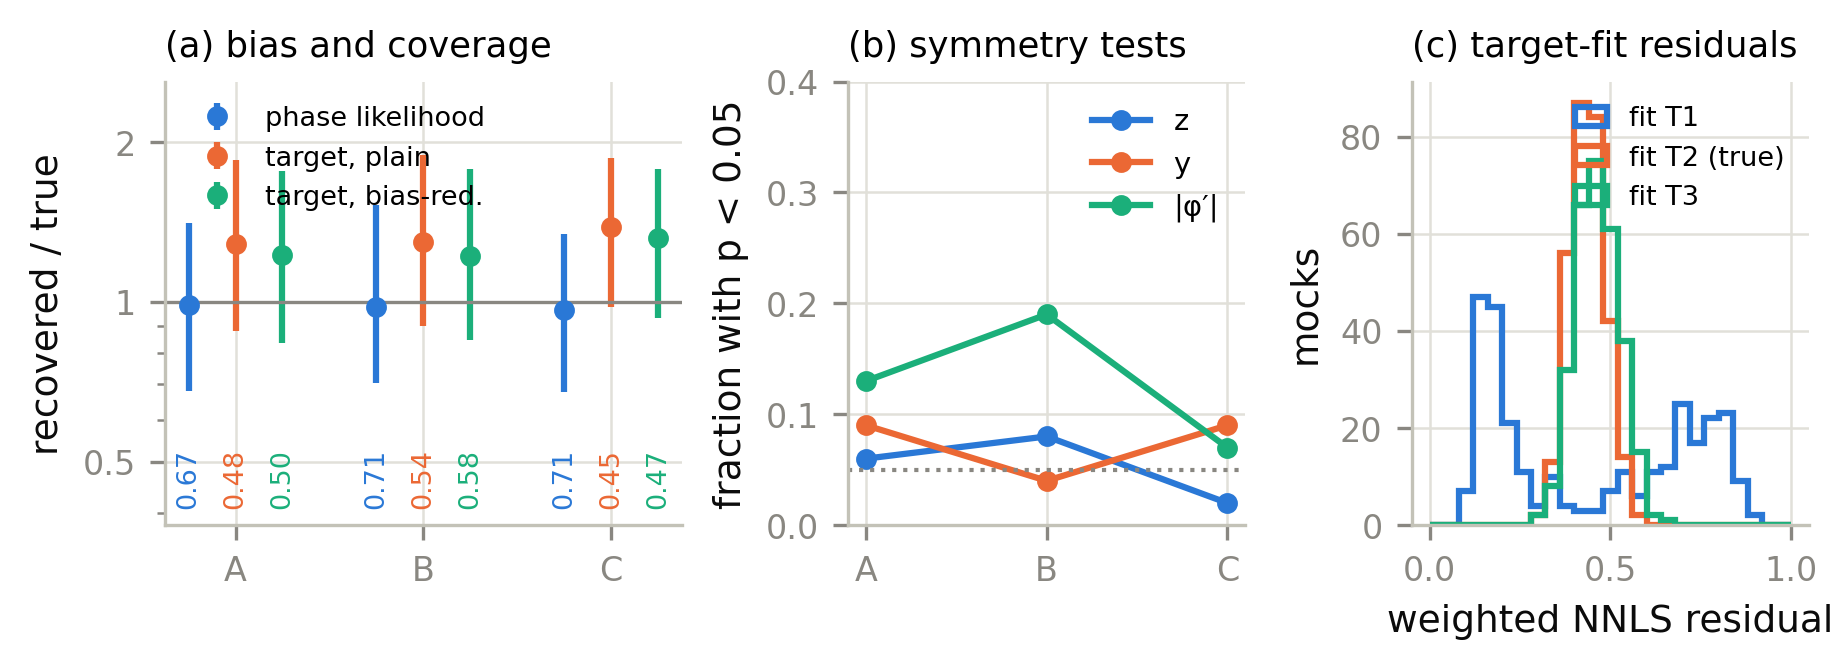
\includegraphics[width=\textwidth]{paper_mock_classes.png}
\caption{Mock validation of the per-class estimators. (a) Recovered/true relative completeness
(median and 16--84\% range) for the phase likelihood and the target estimator, plain and
bias-reduced, in scenarios A--C; the vertical numbers give the 68\% coverage. (b) Fraction of mocks
in which each symmetry test gives $p<0.05$; the dotted line marks 5\%. (c) Target-fit residuals when
the truth is T2; a residual cannot rank targets, since a T1 fit often beats the true T2.}
\label{fig:mock_classes}
\end{figure}

\begin{figure}[p]
\centering
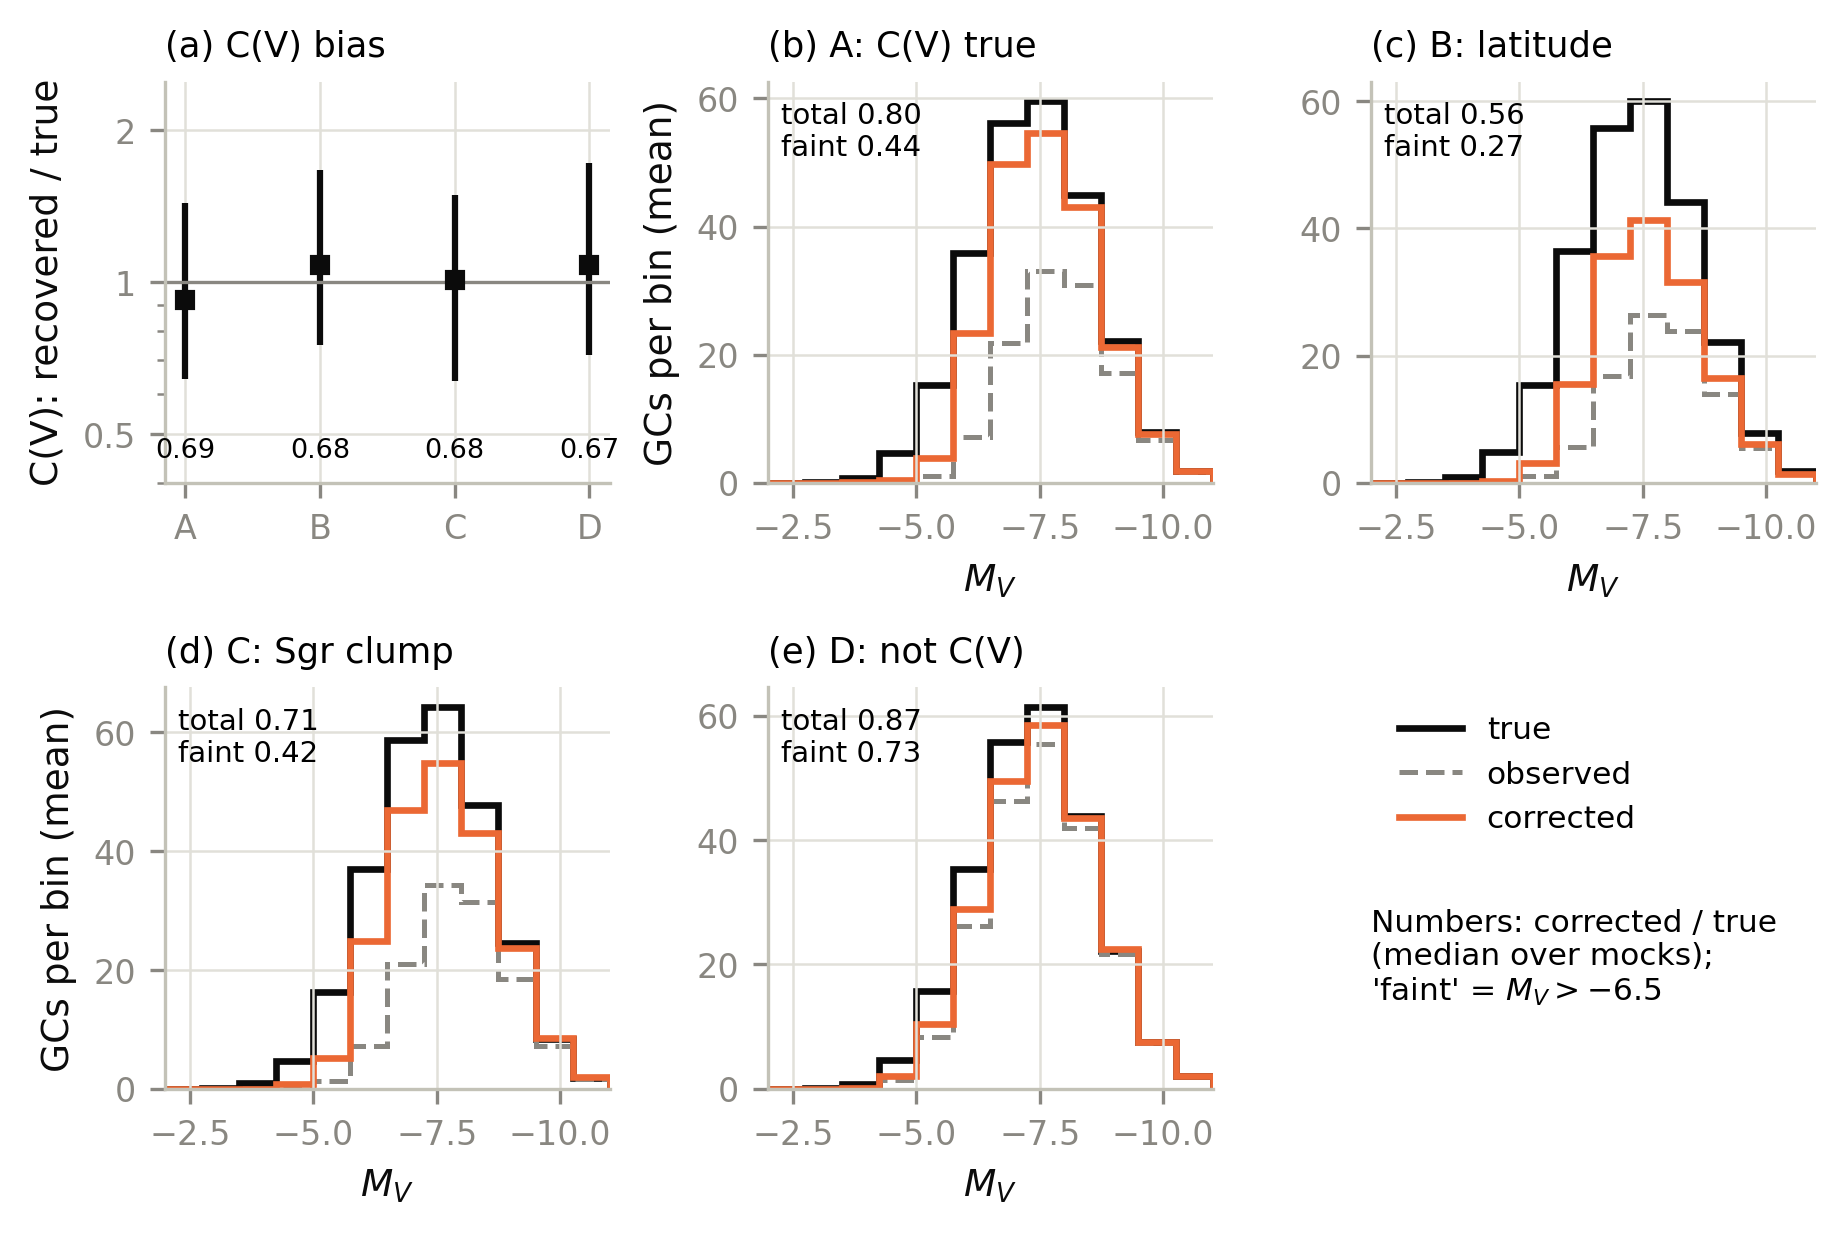
\includegraphics[width=\textwidth]{paper_mock_cv.png}
\caption{Mock validation of $C(V)$. (a) Recovered/true $C(V)$ per bin (median and 16--84\% range)
in scenarios A--D; numbers give the 68\% coverage. (b)--(e) True (black), observed (dashed) and
corrected (orange) $\MV$ distributions, mean over realisations; numbers give the median
corrected/true ratio for all GCs and for $\MV>-6.5$.}
\label{fig:mock_cv}
\end{figure}

%======================================================================
\section{Results}
\label{sec:results}

\subsection{Completeness per luminosity class}

Table~\ref{tab:classes} and Fig.~\ref{fig:classes} give the per-class completeness. In the two
brighter classes completeness stays near unity out to $\approx 10$ kpc and falls to 0.4--0.6
beyond. The faint class drops to $0.44$ already at 8--21 kpc. In-situ clusters lose completeness
steeply with distance (0.18 beyond 8.8 kpc); accreted clusters stay near unity to 27 kpc and fall to
0.27 beyond (Fig.~\ref{fig:pops}). The fixed-target estimator agrees with the phase likelihood within
the intervals in most bins, but for the accreted clusters it gives values above 1 beyond 18 kpc,
which the phase likelihood does not reproduce; these follow from the assumed target shape.

\begin{table}[h]
\centering
\caption{Phase-likelihood completeness relative to the nearest distance bin, with 68\% profile
intervals. Each class holds 55 GCs in three bins of 18--19.}
\label{tab:classes}
\small\setlength{\tabcolsep}{4pt}
\begin{tabular}{lccc}
\toprule
$\MV$ class & nearest bin & second bin & third bin \\
\midrule
$-10.54$ to $-7.58$ & $0$--$8.3$ kpc: 1 & $8.3$--$11.1$ kpc: $1.22\,[0.88, 1.71]$ & $>11.1$ kpc: $0.63\,[0.41, 0.95]$ \\
$-7.58$ to $-6.50$ & $0$--$7.4$ kpc: 1 & $7.4$--$9.5$ kpc: $0.75\,[0.52, 1.07]$ & $>9.5$ kpc: $0.41\,[0.28, 0.61]$ \\
$-6.50$ to $-0.96$ & $0$--$7.8$ kpc: 1 & $7.8$--$21.5$ kpc: $0.44\,[0.31, 0.62]$ & $>21.5$ kpc: $0.56\,[0.27, 1.22]$ \\
\bottomrule
\end{tabular}
\end{table}

\begin{figure}[p]
\centering
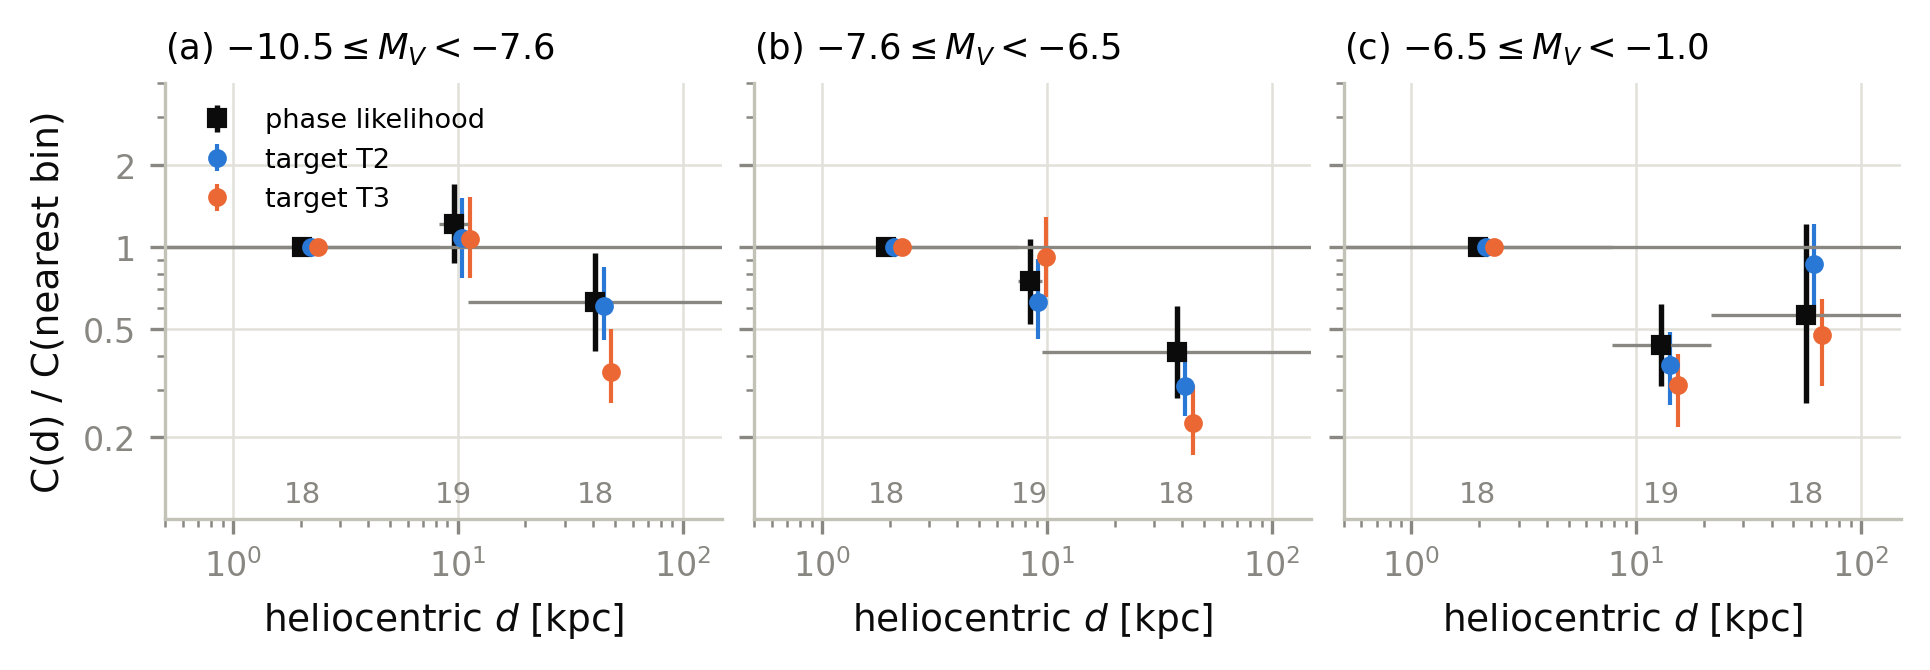
\includegraphics[width=\textwidth]{paper_real_classes.png}
\caption{Completeness relative to the nearest distance bin for three $\MV$ classes: phase likelihood
(black squares, 68\% profile intervals; grey bars show the bin extent) and the fixed-target
estimator for targets T2 and T3 (coloured; bias-reduced, 68\% bootstrap). Numbers give the observed
clusters per bin.}
\label{fig:classes}
\end{figure}

\begin{figure}[p]
\centering
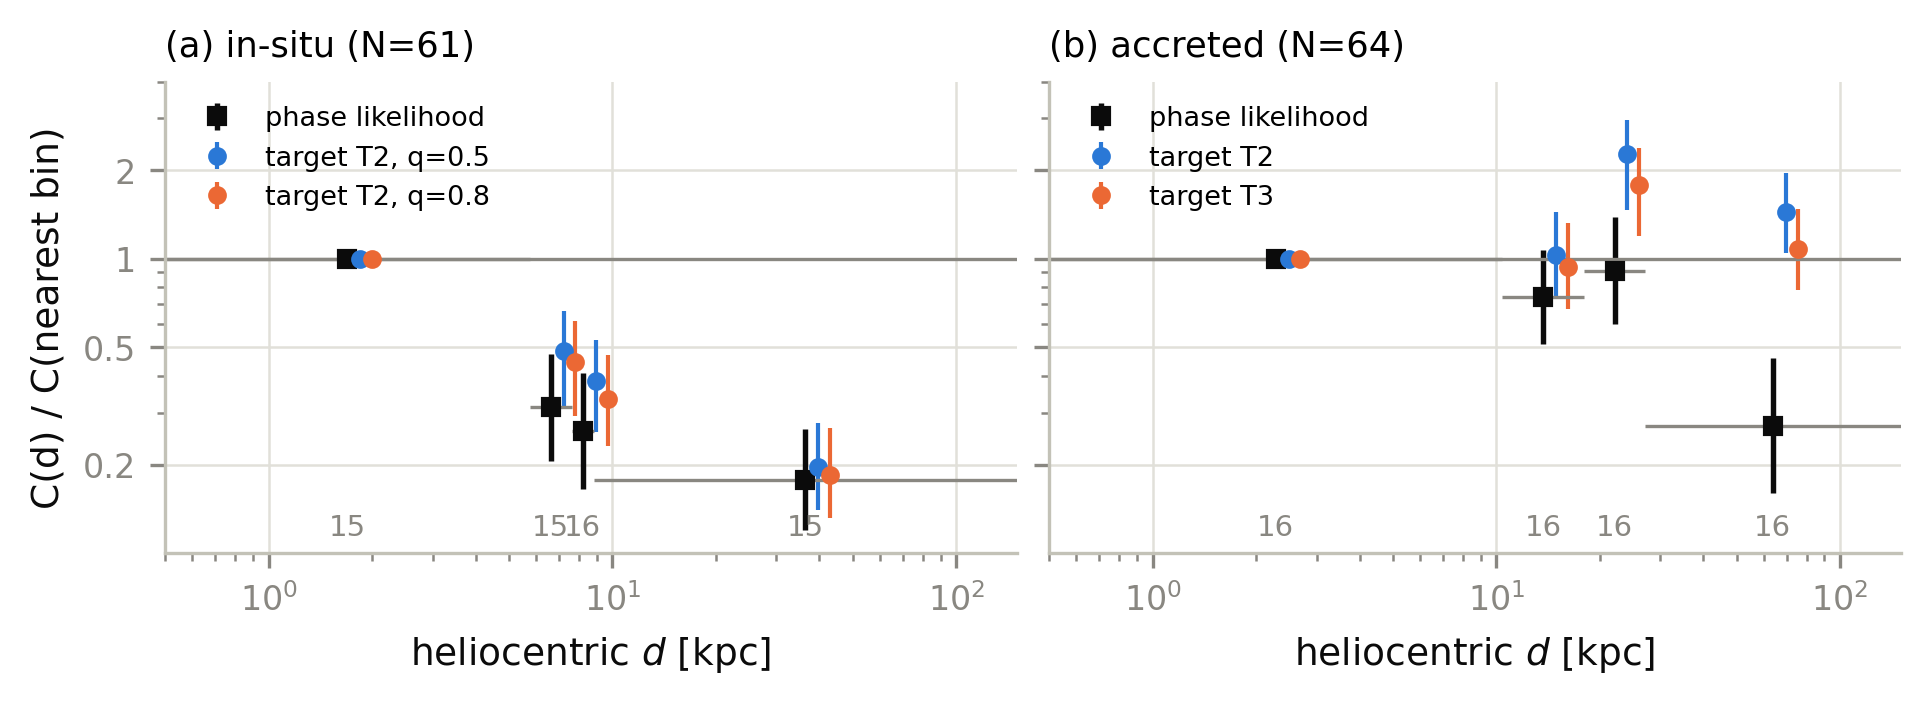
\includegraphics[width=\textwidth]{paper_real_populations.png}
\caption{As Fig.~\ref{fig:classes}, for in-situ (left) and accreted (right) clusters, all
luminosities combined.}
\label{fig:pops}
\end{figure}

\subsection{Symmetry tests}

The pooled PIT tests (Fig.~\ref{fig:sym}) give $p = 0.46$ for $z$, $0.042$ for $y$ and $0.006$ for
$|\phi'|$. Split by population, the in-situ clusters give $p = 0.040$, $0.29$ and $0.006$, and the
accreted clusters $0.51$, $0.49$ and $0.75$. Since null mocks reach $p\le0.01$ for $|\phi'|$ in only
2\% of realisations, the in-situ clusters carry an azimuthal structure that completeness depending
on $(\MV,\dhel)$ alone does not explain. The Galactic bar, which this analysis does not mask, is one
candidate. The data do not identify the cause.

\begin{figure}[h]
\centering
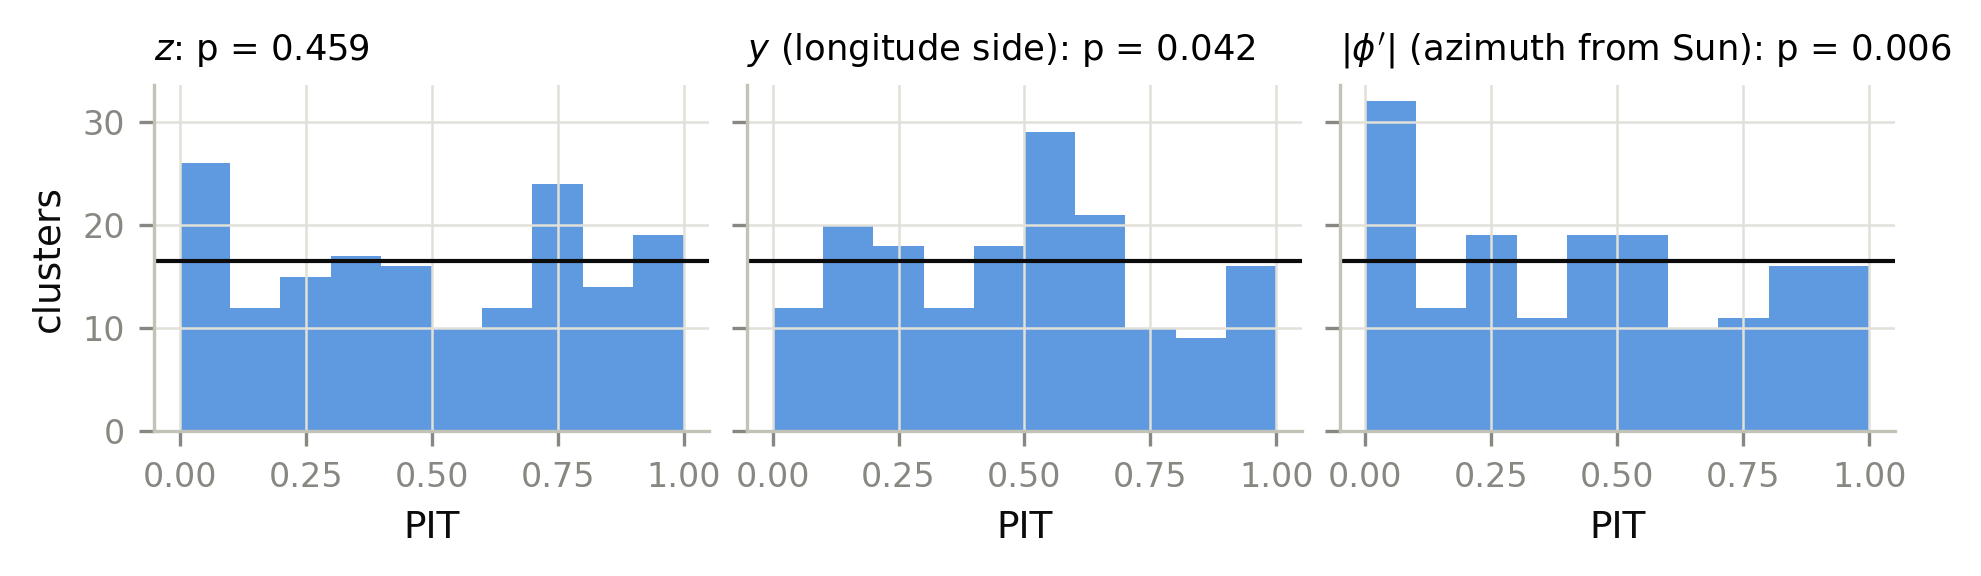
\includegraphics[width=\textwidth]{paper_real_symmetry.png}
\caption{Pooled PIT values for $z$, $y$ and $|\phi'|$ against each orbit's $C$-weighted phase
distribution. Uniform histograms are expected if the model holds; the titles give the KS statistic
and the null-calibrated $p$-value.}
\label{fig:sym}
\end{figure}

\subsection{Completeness versus apparent magnitude}

Table~\ref{tab:cv} and Fig.~\ref{fig:cv} give $C(V)$. Completeness falls steadily from unity at
$V<6$ to $0.14\,[0.07,0.30]$ at $V>11$. The per-class completeness curves implied by $C(V)$ follow
the free per-class fits (Fig.~\ref{fig:cv}, right), and the AIC prefers $C(V)$ ($-6.0$ against
$-1.5$), although the mocks show this comparison is weak.

\begin{table}[h]
\centering
\caption{$C(V)$ from the phase likelihood (brightest bin fixed at 1); 68\% profile intervals. Each bin
holds 20--21 GCs.}
\label{tab:cv}
\small\setlength{\tabcolsep}{4pt}
\begin{tabular}{lcccccccc}
\toprule
$V$ & $<6.0$ & $6.0$--$6.6$ & $6.6$--$7.2$ & $7.2$--$7.6$ & $7.6$--$8.2$ & $8.2$--$9.2$ & $9.2$--$11.0$ & $>11.0$ \\
\midrule
$C$ & 1 & $1.17$ & $0.56$ & $0.64$ & $0.41$ & $0.25$ & $0.21$ & $0.14$ \\
68\% & -- & $[0.82, 1.68]$ & $[0.38, 0.82]$ & $[0.43, 0.95]$ & $[0.27, 0.62]$ & $[0.16, 0.39]$ & $[0.13, 0.35]$ & $[0.07, 0.30]$ \\
\bottomrule
\end{tabular}
\end{table}

\begin{figure}[h]
\centering
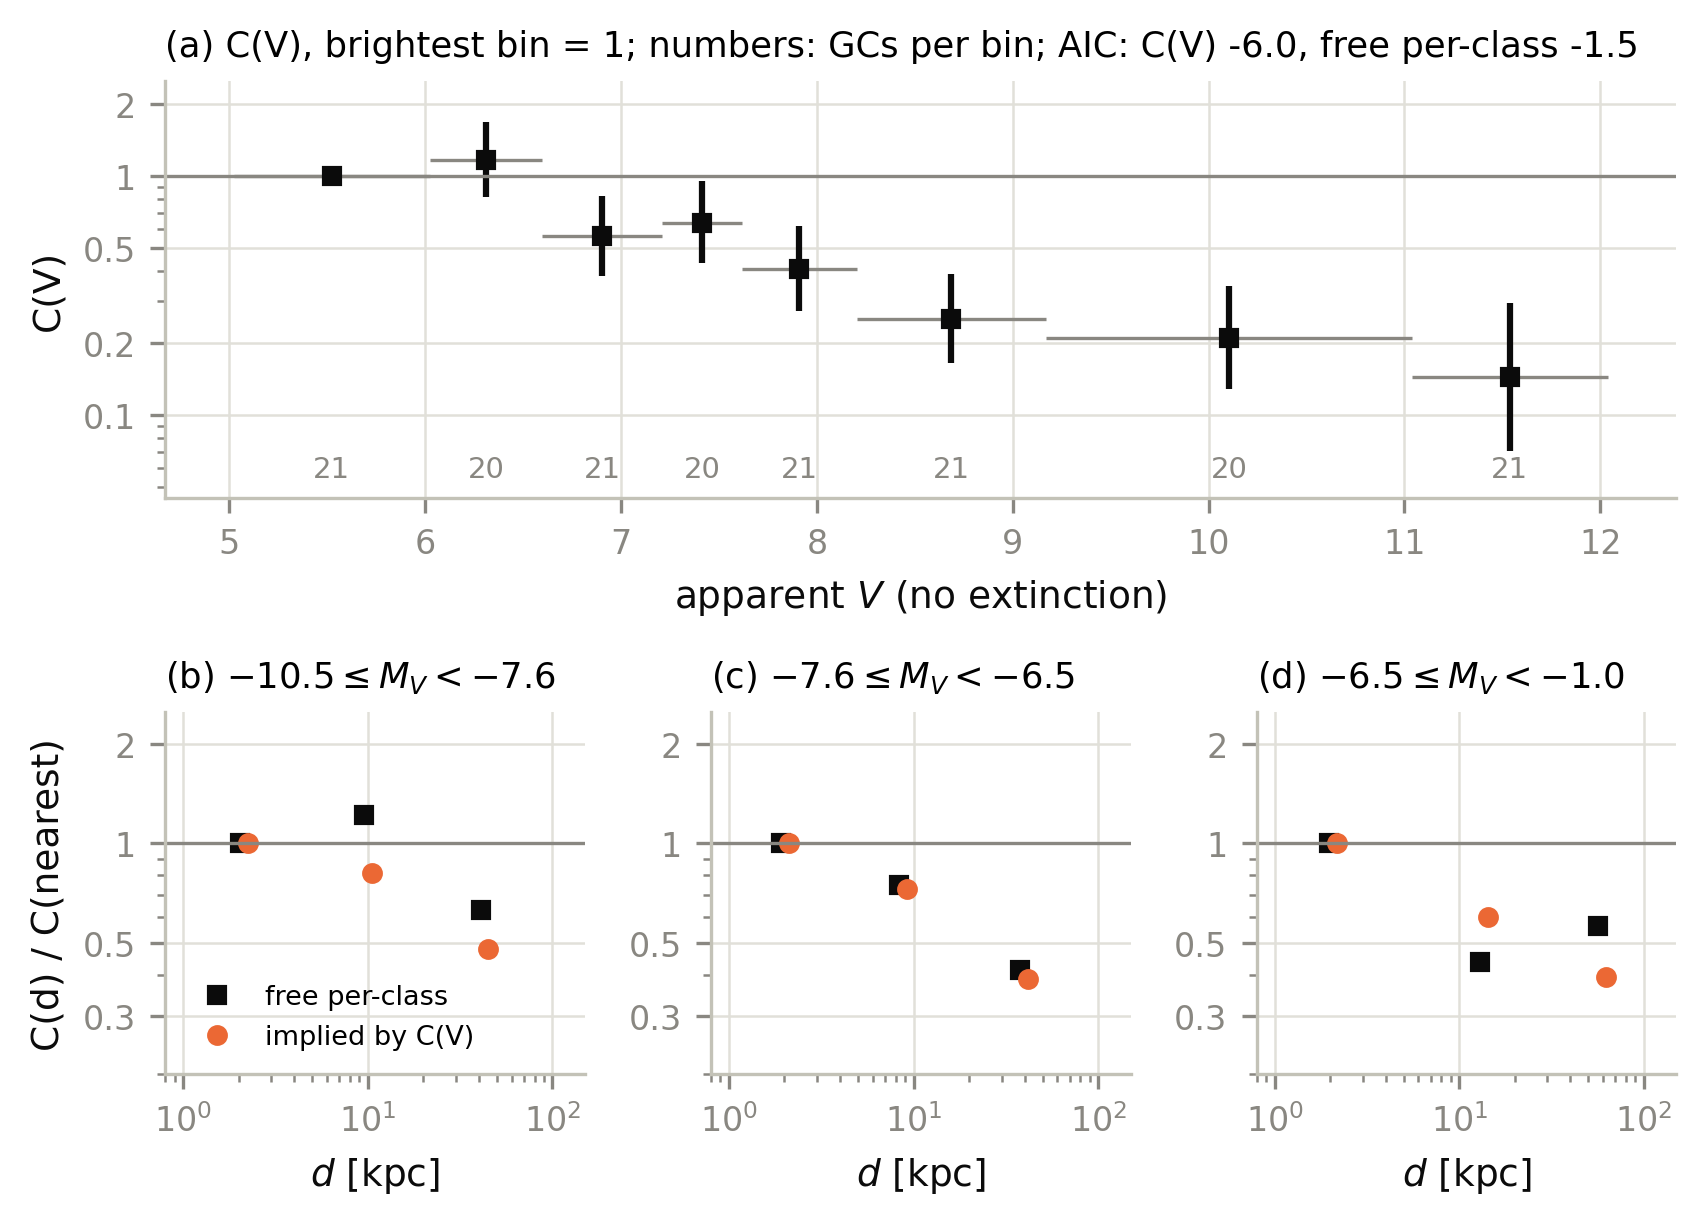
\includegraphics[width=\textwidth]{paper_real_cv.png}
\caption{(a) $C(V)$ with 68\% profile intervals; grey bars show the bin extent and numbers give
clusters per bin. (b)--(d) Per-class completeness versus distance from free fits (black) and
implied by $C(V)$ (orange).}
\label{fig:cv}
\end{figure}

\subsection{Corrected luminosity and metallicity distributions}

Weighting by $1/q_i$ (weights from $0.94$ to $6.9$) turns the 165 observed GCs into $483$
($68\%$: $335$--$765$). The correction grows with faintness (Fig.~\ref{fig:corr}): bright clusters
($\MV<-8$) rise from 40 to 60, intermediate ones ($-8\le\MV<-6.5$) from 70 to 156, and faint ones
($\MV\ge-6.5$) from 55 to 267 ($168$--$473$). The corrected metallicity distribution is about three
times the observed one at all $\feh$ and keeps its bimodal shape, with peaks near $-1.5$ and $-0.6$.
Given Sec.~\ref{sec:mocks}, these corrected numbers are lower limits if the real selection
resembles the mocks.

\begin{figure}[h]
\centering
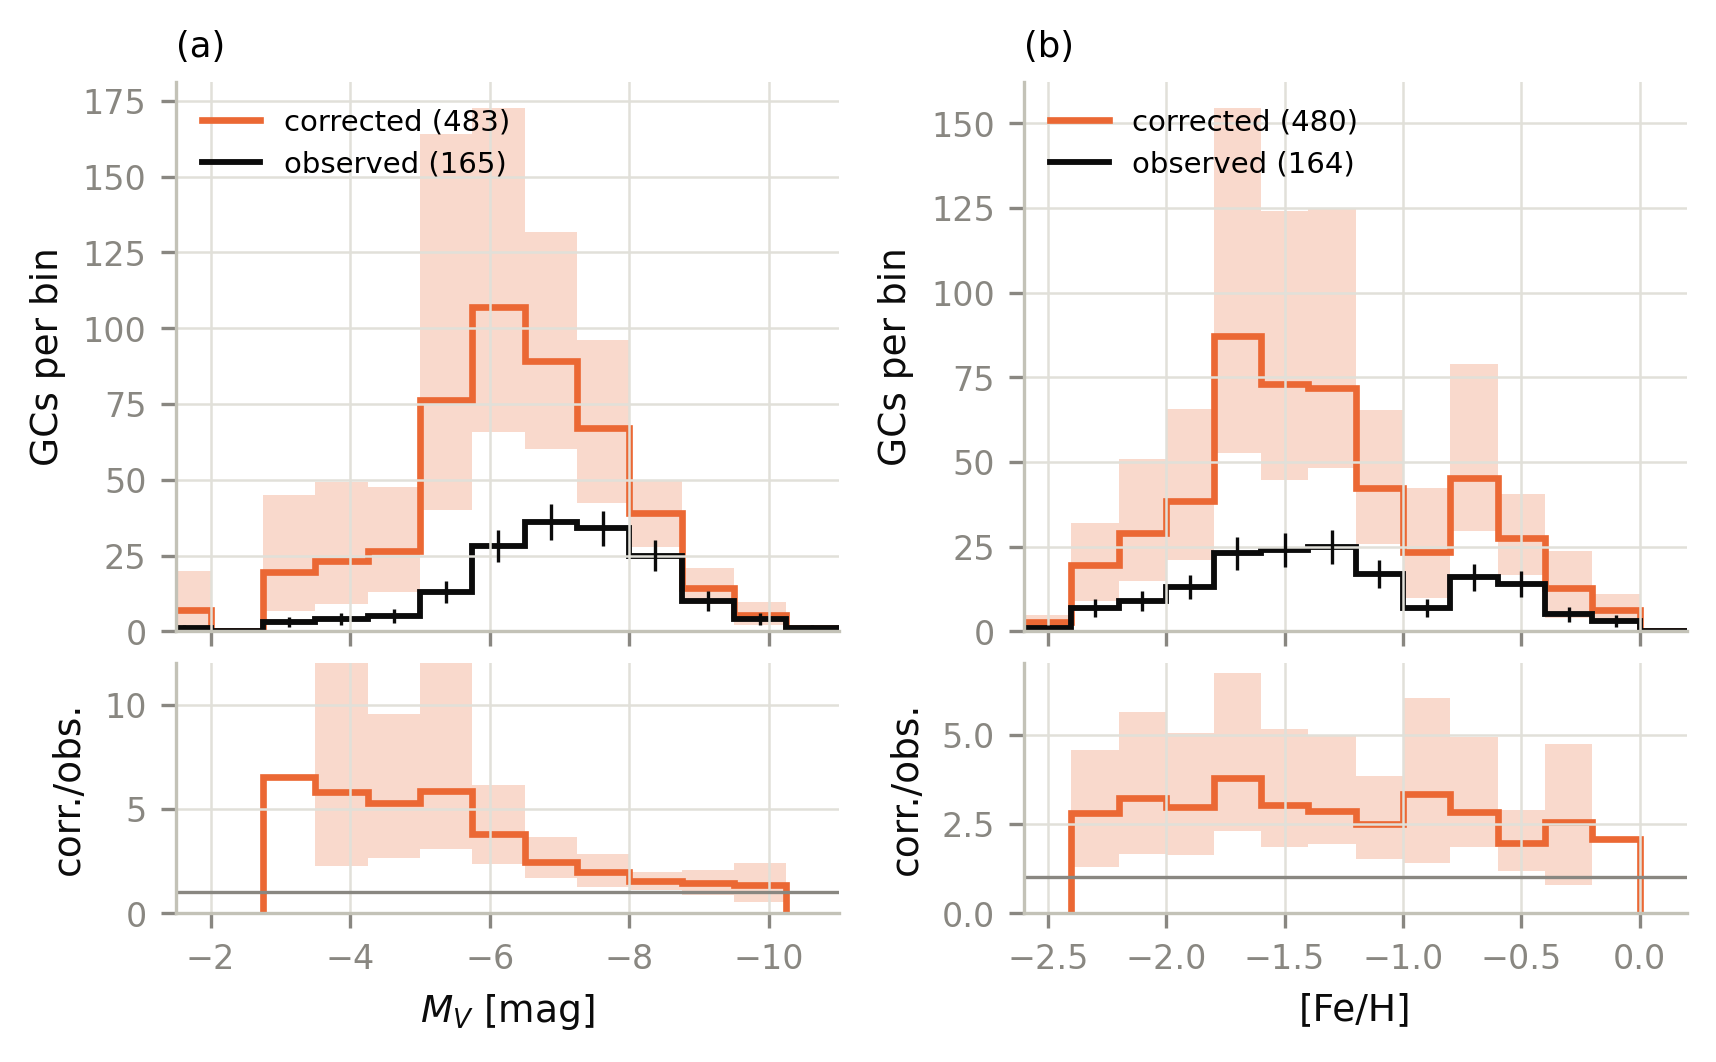
\includegraphics[width=\textwidth]{paper_corrected.png}
\caption{Observed (black) and completeness-corrected (orange, 68\% bootstrap band) $\MV$ and $\feh$
distributions using $C(V)$. Lower panels: corrected/observed.}
\label{fig:corr}
\end{figure}

\subsection{Why extinction matters, and what the mocks show}
\label{sec:whydust}

Whether a cluster is found depends on how bright it looks, and dust makes it look fainter: the
relevant apparent magnitude is $V + A_V$, not $V$. Dust is concentrated in the Galactic disc, and
most GCs live in the inner Galaxy, where many sightlines cross the disc and the bulge. The
catalogue's present-day reddenings reach $E(B-V) = 6.8$, i.e.\ $A_V \approx 21$ mag, and half the
clusters have $A_V > 1$ mag.

Extinction enters the phase likelihood in two places.
\begin{enumerate}
\item \textbf{The shape of $C$.} Along an orbit a cluster's brightness changes not only with distance
but also with the sightline: passing behind the bulge it can dim by several magnitudes at almost
the same distance. If $A_V$ is left out, the fit can only attribute that dimming to distance or
luminosity, which distorts $C(V)$.
\item \textbf{The corrected counts.} An orbit that spends time behind thick dust is detectable for a
smaller fraction of its period. Ignoring the dust overestimates its orbit-averaged completeness
$q_i$, so its weight $1/q_i$ is too small and the counts are under-corrected.
\end{enumerate}
Because extinction depends on direction as well as distance, it also breaks the assumption that
completeness depends on $\MV$ and $\dhel$ alone, unless it is folded into $V$.

To test this we added a mock scenario (E) in which detection depends on $V + A_V$, with $A_V$
computed along every orbit from an exponential dust disc ($A_V$ of 1 mag kpc$^{-1}$ in the plane at
the solar circle, radial scale 3 kpc, vertical scale 0.1 kpc). We then fit each mock twice: with the
true $A_V$ added to $V$, and ignoring dust. Over 100 realisations:
\begin{itemize}
\item \textbf{The completeness curve is recovered when dust is included:} recovered/true $C(V+A_V)$
is $1.00$, with 68\% coverage $0.62$.
\item \textbf{Including dust reduces the bias in the corrected counts, but does not remove it:} the
corrected total is $0.61$ of the truth with the correct $A_V$ and $0.51$ ignoring dust; for faint
clusters ($\MV>-6.5$) the figures are $0.18$ and $0.16$. The remaining shortfall is the
unseen-orbit limitation of Sec.~\ref{sec:mocks}, which dust makes worse because it hides more
orbits entirely: only 6\% of the faint mock clusters are detected.
\item \textbf{The likelihood can tell a correct dust model from no dust:} the AIC favours the true
extinction model over ignoring dust in 98\% of the realisations.
\end{itemize}
The last point matters for the real data. The likelihood comparison is a sensitive test, so the
preference for no extinction over the present-day-reddening model in Sec.~\ref{sec:ext} is evidence
against that particular model, rather than against the importance of dust. Separately, mock
scenario B, whose latitude-dependent selection mimics dust that the model does not include, biases
the corrected total low (0.56 of the truth).

\subsection{Extinction: present-day reddening, 3D maps, and simple proxies}
\label{sec:ext}

We tested three treatments of dust, each compared with the no-dust $C(V)$ fit by AIC
(Table~\ref{tab:dust}).

\paragraph{Present-day reddening held fixed.} Adding $A_V = 3.1\,E(B-V)$, with each cluster's
catalogue reddening at its present position held fixed along its whole orbit, raises the totals to
689 ($457$--$1172$) and 337 ($203$--$651$) faint. The data disfavour this model (AIC $+1.3$ against
$-6.0$ without dust). Holding present reddening fixed while a cluster moves to other sightlines is
unphysical; this test shows only that the total is sensitive, by about 43\%, to an untested
prescription.

\paragraph{3D dust maps along each orbit.} We evaluate extinction at every one of the
$165\times500$ orbit samples with the \texttt{dustmaps} package. The maps are combined by priority:
DECaPS 3D (Zucker et al.\ 2025; southern plane $239^\circ<l<6^\circ$, $|b|<10^\circ$, reliable to
10 kpc), then Bayestar19 (Green et al.\ 2019; where flagged reliable), then Marshall et al.\ (2006;
inner plane, within each sightline's last distance slice), and SFD (Schlegel et al.\ 1998) otherwise. DECaPS supplies
$A_V$ for 24\% of the orbit samples, Marshall for 13\%, Bayestar19 for 8\% and SFD for the remaining
55\%, mostly at high latitude. Conversions: $A_V = 3.1\,E(B-V)$ for DECaPS and Bayestar19
($E(B-V) = 0.883\times$ the Bayestar19 value), $A_V = 8.8\,A_{K_s}$ for Marshall, and
$A_V = 2.742\,E(B-V)_{\rm SFD}$ (Schlafly \& Finkbeiner 2011). Beyond a 3D map's reliable distance
the true $A_V$ is bracketed: the low bracket keeps the map's last value (no more dust), the high
bracket uses the SFD total of the sightline (all its dust in front). At the clusters' present
positions the maps give 5--8\% less extinction than the catalogue reddening (median map/catalogue ratio 0.92 and 0.95 for the low and high brackets, 144 clusters with catalogue $A_V>0.1$).

This model fits the data best (AIC $-13.7$ and $-14.4$ for the two brackets, against $-6.0$
without dust). Since the mocks show the likelihood picks the correct dust model in 98\% of
realisations (Sec.~\ref{sec:whydust}), the improvement is meaningful. The corrected total
\emph{falls} to 411--455, with tighter intervals, and the faint count to 197--218
(Fig.~\ref{fig:ext}). Accounting for dust lets distant clusters behind it count as dimmed rather
than distant, which changes the shape of $C$. With dust, the correction for metal-poor clusters
($\feh<-1$) drops from $\times3.1$ to $\times2.4$, while that for metal-rich clusters stays at
$\times2.6$, so the two now receive similar corrections.

\paragraph{Simple obscuration proxies.} Without 3D maps, obscuration can be fitted directly: we write
$C = C_V(V)\,g(x)$, with $x$ either $|b|$ or the 2D SFD reddening of the sightline at each orbit
sample, and $g$ a step function in three equal-count bins anchored to 1 in the least obscured bin.
The phase likelihood learns $g$ from where along their orbits the clusters are caught. On mocks
(Table~\ref{tab:proxy}) the proxies do no harm when there is no obscuration and reduce the
shortfall when there is; the AIC prefers them over $C(V)$ in 12--15\% of null mocks and in 69--71\%
of the dust mocks. On the real data, $g(|b|)$ fits better than no dust (AIC $-10.4$), with clusters
in the lowest-$|b|$ third detected about half as often ($g = 0.49$), and gives a corrected total of
520; the 2D-SFD proxy is weaker (AIC $-7.5$; total 462).

\begin{table}[h]
\centering
\caption{Real data: dust treatments compared. AIC is relative to the same data (lower is better);
totals and faint counts ($\MV>-6.5$) with 68\% bootstrap intervals.}
\label{tab:dust}
\small\setlength{\tabcolsep}{4pt}
\begin{tabular}{lccc}
\toprule
Model & AIC & Corrected total & Faint \\
\midrule
No extinction, $C(V)$ & $-6.0$ & 483 ($335$--$765$) & 267 ($168$--$473$) \\
Present $E(B-V)$ fixed along orbit & $+1.3$ & 689 ($457$--$1172$) & 337 ($203$--$651$) \\
Proxy $C_V(V)\,g(E(B-V)_{\rm SFD})$ & $-7.5$ & 462 ($346$--$668$) & 251 \\
Proxy $C_V(V)\,g(|b|)$ & $-10.4$ & 520 ($400$--$753$) & 269 \\
3D maps along orbits, low bracket & $-13.7$ & 455 ($354$--$634$) & 218 ($158$--$327$) \\
3D maps along orbits, high bracket & $\mathbf{-14.4}$ & 411 ($319$--$566$) & 197 ($140$--$291$) \\
\bottomrule
\end{tabular}
\end{table}

\begin{table}[h]
\centering
\caption{Mocks: corrected total / true (faint in brackets), median over 100 realisations, for
$C(V)$ alone and the two proxy models. In scenario E, the $C(V)$ column ignores dust; with the
true $A_V$ supplied, the total is 0.61 (faint 0.18).}
\label{tab:proxy}
\small\setlength{\tabcolsep}{4pt}
\begin{tabular}{lccc}
\toprule
Scenario & $C(V)$ & $C_V(V)\,g(|b|)$ & $C_V(V)\,g(\text{2D column})$ \\
\midrule
A: no obscuration & $0.80$ ($0.44$) & $0.83$ ($0.43$) & $0.82$ ($0.41$) \\
B: latitude-dependent selection & $0.56$ ($0.27$) & $0.64$ ($0.31$) & $0.65$ ($0.31$) \\
E: dust disc & $0.51$ ($0.16$) & $0.68$ ($0.19$) & $0.69$ ($0.19$) \\
\bottomrule
\end{tabular}
\end{table}

\begin{figure}[h]
\centering
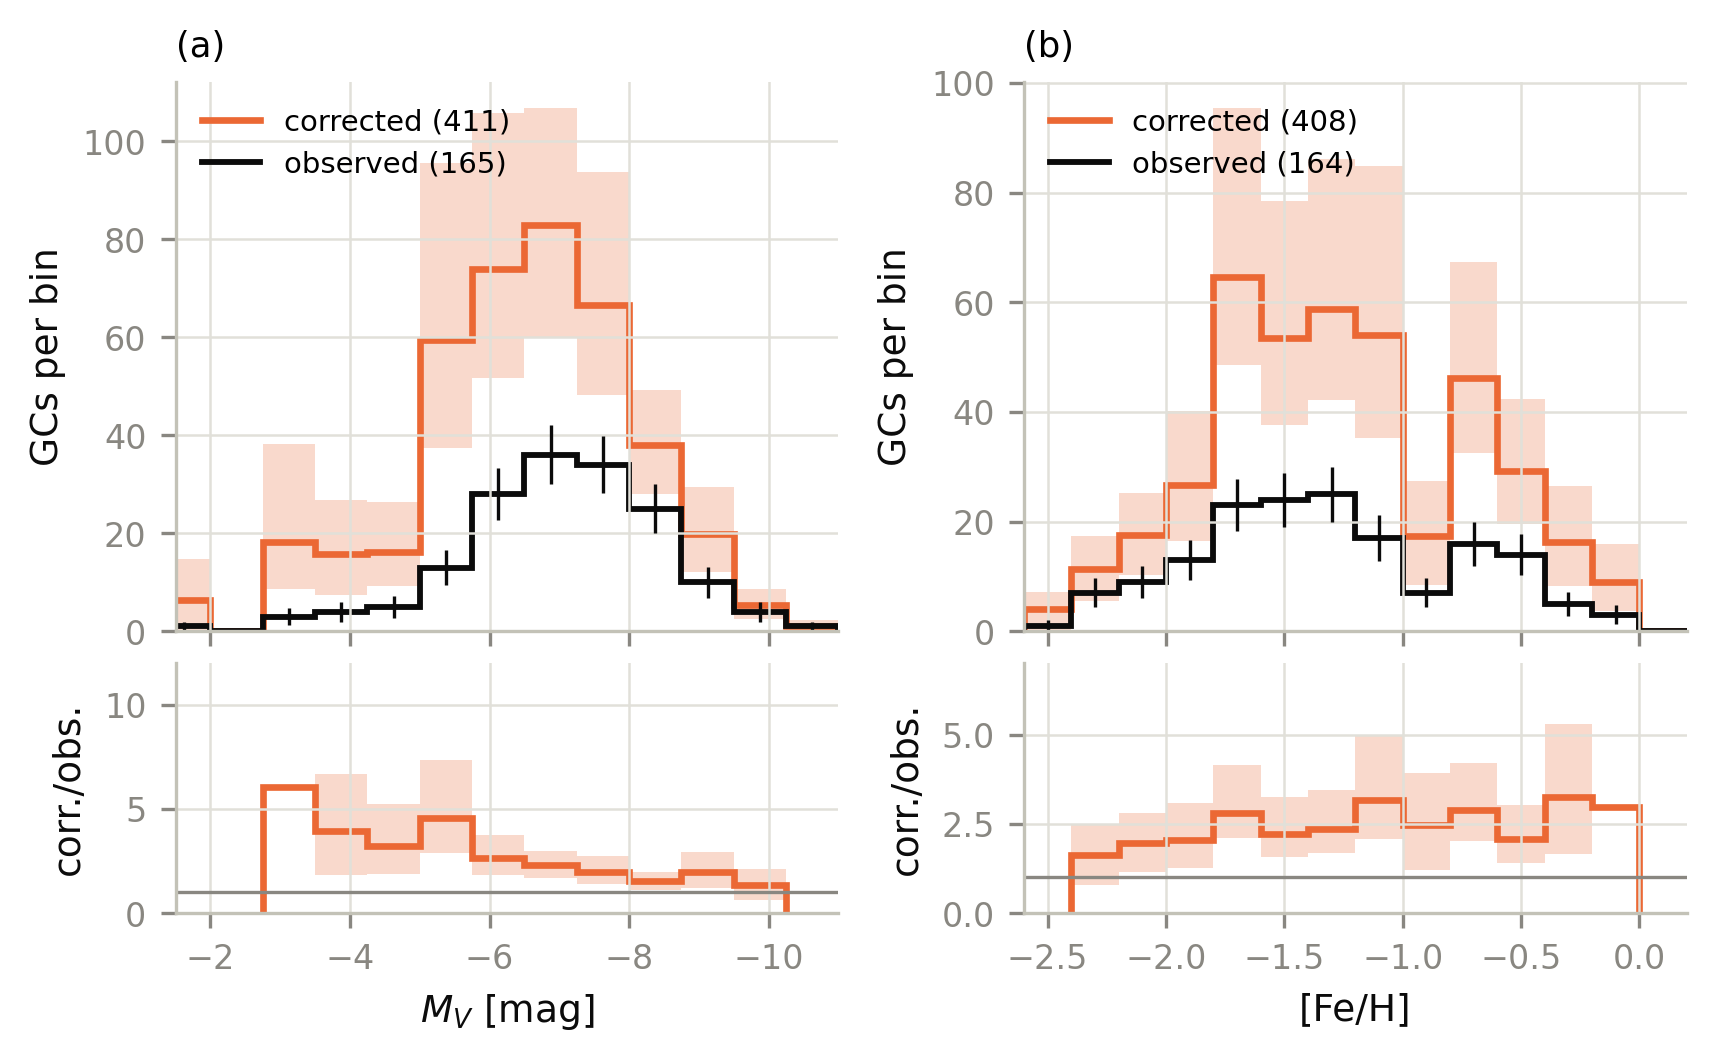
\includegraphics[width=\textwidth]{paper_corrected_map_high.png}
\caption{As Fig.~\ref{fig:corr}, with $A_V$ from 3D dust maps evaluated along every orbit
(high bracket, the best-fitting binned model).}
\label{fig:ext}
\end{figure}

\subsection{Why the no-dust fit overcorrects: the inner Galaxy's dust applied to the halo}
\label{sec:nodustbias}

Adding dust to the model \emph{lowers} the corrected total (483 to 411--455 binned, 749 to 432--461
continuous), although dust makes clusters fainter. The reason is that the no-dust fit is not free of
dust: it absorbs the dust losses of the inner Galaxy into $C(V)$ and then applies them in every
direction.

\paragraph{Where the signal comes from.} If a cluster is detected with equal probability all along
its orbit and is phase-mixed, the fraction $u_i$ of its orbit time spent closer to the Sun than it is
now is uniform on $[0,1]$. For the 43 GCs at $\dhel>15$ kpc the median $u$ is 0.44 and a KS test
against uniform gives $p=0.79$: within their own orbits, the halo clusters show no sign of
incompleteness. For the 122 GCs at $\dhel<15$ kpc the median is 0.32 ($p=6\times10^{-9}$): they are
caught preferentially at the near parts of their orbits. These are the inner clusters whose orbits
cross the disc and bulge. With the 3D maps, the 68 clusters whose orbits have a median galactocentric
radius below 4 kpc have an orbit-averaged $A_V$ of 3.6 mag (median) and spend 39\% of their time
behind $A_V>3$. At their present positions the median is only 1.7 mag: they are caught in the less
obscured parts of their orbits.

\paragraph{How the no-dust fit uses it.} Without $A_V$, the likelihood can attribute that deficit only to
$V$, so $C(V)$ falls steeply over $V\approx7$--11, the range the inner orbits span. That steep curve
also applies to halo clusters at the same $V$, on dust-free sightlines. Halo clusters whose whole orbit
lies at $V>11$ (Pal~3, Pal~4, Crater, AM~4, Whiting~1 and others) all get the largest weight,
$1/C_{\rm last} = 1/0.144 = 6.9$. With the maps the curve becomes shallower, their $q$ rises to
0.18--0.20 and their weights fall to 5.0--5.5, while the dust loss lands on the orbits that actually
cross the dust.

Table~\ref{tab:nodust} splits the change into two steps. Refitting $C$ with the maps but switching
the dust off along the orbits shows how much loss the no-dust curve had absorbed: all weights fall.
Switching the dust back on restores the loss where it belongs: the inner weights double, the outer
ones partly recover. Net, the inner clusters gain 19 and the outer ones lose 89. By present
extinction: clusters with $A_{V,\rm now}<1$ (84) go from a summed weight of 296 to 207, those with
$A_{V,\rm now}>1$ (81) from 187 to 204; the most obscured bulge clusters change most (Terzan~5, $q$
from 1.00 to 0.21; Terzan~1, 0.96 to 0.16).

\begin{table}[h]
\centering
\caption{Summed weights $\sum 1/q_i$ (binned $C$) for clusters whose orbits have median galactocentric
radius below 4 kpc (inner) or above (outer). (a) no-dust fit $C_0(V)$; (b) $C$ refitted with map
extinction (high bracket) but evaluated without $A_V$ along the orbits; (c) the map fit, $C_d(V+A_V)$.}
\label{tab:nodust}
\small
\begin{tabular}{lccc}
\toprule
 & Inner (68) & Outer (97) & Total \\
\midrule
(a) $C_0(V)$, no dust & 152 & 330 & 483 \\
(b) $C_d(V)$, dust off along orbits & 86 & 200 & 287 \\
(c) $C_d(V+A_V)$ & 171 & 241 & 411 \\
\bottomrule
\end{tabular}
\end{table}

\paragraph{Why mock E behaves differently.} In mock scenario E, ignoring dust lowers the corrected total
(0.51 against 0.61 of truth with the true $A_V$). The sign of the bias depends on the balance between
the two terms: the extra loss on dusty orbits, which ignoring dust misses, and the steepened $C(V)$
applied to dust-free orbits at the same $V$. In the mock population the first dominates; in the real
catalogue, where the largest weights belong to distant halo clusters, the second does. The
likelihood settles which model is right in either case: it prefers the map model by $\Delta{\rm AIC}
= 8$ (binned) and 16--17 (continuous), and in mocks it picks the true dust model in 98\% of realisations.

\subsection{Faint clusters on never-detectable orbits: continuous $C(V)$ and $1/V_{\max}$}
\label{sec:vmax}

\paragraph{Two sources of the faint-end shortfall.} Mock tests isolate two causes of the low corrected
counts in Table~\ref{tab:mock_cv}. With the true $C$, the own-orbit weights $1/q_i$ recover 87\% of the
total and 63\% of the faint clusters (scenario A, median of 8 realisations): the rest are clusters
whose $q_i$ is nearly zero. With the fitted binned $C$ the faint fraction falls to 41\%. The last
$V$ bin is open, so the binned model holds $C$ constant at all fainter $V$, where the true $C$ falls to
zero. This inflates $q_i$ for faint clusters, whose orbits spend most of their time beyond the
faintest detection. Even the best binned $C$ (its pseudo-true value) recovers only 36\% of the faint
clusters.

\paragraph{Continuous $C(V)$.} We therefore also fit $\ln C$ as a piecewise-linear function of $V$,
with nodes at the median observed $V$ of the same eight equal-count bins. It is anchored to $C=1$ at
the brightest node and held flat at brighter $V$, and beyond the faintest node it continues with the
last slope, constrained to be $\le 0$. The model has the same seven parameters as the binned one and
is fitted with the same likelihood (Eq.~\ref{eq:phaselike}).

\paragraph{$1/V_{\max}$ over the orbit population.} We assume the orbit distribution of GCs does not
depend on luminosity. Bright clusters ($\MV<-8$) are detectable along essentially all orbits, so their
$1/q$-weighted orbits sample the orbit population. A cluster of absolute magnitude $M$ placed at a
random phase on that population is detected with probability
\begin{equation}
f(M) = \frac{\sum_{j:\,\MV<-8} q_j^{-1}\,\langle C(M+\mu_j(t))\rangle_t}{\sum_{j:\,\MV<-8} q_j^{-1}},
\qquad \mu_j(t) = 5\log_{10}\frac{d_j(t)}{10\,\mathrm{pc}} + A_{V,j}(t),
\end{equation}
and each observed cluster gets weight $1/f(M_{V,i})$ in place of $1/q_i$. This is the
$1/V_{\max}$ estimator (Schmidt 1968) with the survey volume replaced by the orbit population. It
counts faint clusters on orbits that no observed faint cluster occupies. For the split by
metallicity we apply the assumption within each class ($\feh<-1$, $\ge-1$), using the bright
clusters of the same class (31 and 9) as its orbit population.

\paragraph{Mock validation.} Table~\ref{tab:vmax_mock} adds two scenarios whose true $C(V)$ is not
log-linear in the tail: F, a shallow all-sky survey plus a deep partial-area survey,
$C = 0.8\,\ell(8,0.3) + 0.2\,\ell(13,0.3)$ with $\ell(V_0,w) = [1+e^{(V-V_0)/w}]^{-1}$; and G, a
power-law tail, $C = (1+V-7)^{-2}$ for $V>7$. The continuous model with $1/V_{\max}$ recovers 0.89--1.13
of the true total and 0.80--1.03 of the faint clusters in every scenario that satisfies its
assumptions (A, C, D, F, G). In scenario E, with the true $A_V$ supplied, it recovers 0.95 of the
total and 0.68 of the faint clusters. It fails, as expected, under the unmodelled latitude selection
of B (0.73 and 0.65). The price is variance: across realisations the total ranges over 0.67--1.55 of
truth (16--84\%, scenario A), and the 68\% bootstrap intervals cover the truth in 53--70\% of mocks,
so they are somewhat too narrow. The continuous model is preferred by AIC in 55--100\% of mocks.

\begin{table}[h]
\centering
\caption{Mocks: corrected total / true (faint, $\MV>-6.5$, in brackets), median of 100 realisations.
Binned: current $C(V)$ with $1/q$. Continuous: $\ln C$ piecewise linear with an extrapolated tail,
with own-orbit $1/q$ or with $1/V_{\max}$. In E, the true $A_V$ is supplied.}
\label{tab:vmax_mock}
\small\setlength{\tabcolsep}{4pt}
\begin{tabular}{lccc}
\toprule
Scenario & Binned, $1/q$ & Continuous, $1/q$ & Continuous, $1/V_{\max}$ \\
\midrule
A: $C(V)$ logistic & 0.80 (0.44) & 1.00 (0.83) & 1.01 (0.95) \\
B: latitude term & 0.56 (0.27) & 0.74 (0.52) & 0.73 (0.65) \\
C: Sgr-like clump & 0.71 (0.42) & 0.96 (0.76) & 1.06 (1.03) \\
D: $C$ not a function of $V$ & 0.87 (0.73) & 0.88 (0.72) & 0.89 (0.81) \\
E: dust disc & 0.61 (0.18) & 0.85 (0.50) & 0.95 (0.68) \\
F: two surveys & 0.94 (0.79) & 1.12 (1.05) & 1.13 (0.98) \\
G: power-law tail & 0.75 (0.39) & 1.04 (0.92) & 0.91 (0.80) \\
\bottomrule
\end{tabular}
\end{table}

\paragraph{Real data.} The continuous model fits better than the binned one: AIC $-22.6$ against
$-14.4$ with the map extinction (high bracket), $-23.7$ against $-13.7$ (low bracket), and $-6.9$
against $-6.0$ without extinction. Table~\ref{tab:vmax_real} gives the corrected counts.
With the maps, $1/V_{\max}$ gives a total of 393 ($274$--$573$) to 418 ($293$--$625$) and 177--189 faint
clusters, close to the binned estimates of Table~\ref{tab:dust} (411--455; 197--218). By metallicity,
the per-class $1/V_{\max}$ gives 245--259 metal-poor and 160--175 metal-rich clusters, against 289--320
and 120--133 with the binned model. The bright metal-rich clusters lie on inner, dusty orbits, so a
faint metal-rich cluster on such an orbit is rarely detectable (Fig.~\ref{fig:vmax}).

\begin{table}[h]
\centering
\caption{Real data, continuous $C(V)$: corrected counts with 68\% bootstrap intervals. Faint:
$\MV\ge-6.5$. $1/V_{\max}$ by [Fe/H] uses the bright clusters of the same class as orbit population.}
\label{tab:vmax_real}
\small\setlength{\tabcolsep}{3pt}
\begin{tabular}{lccc}
\toprule
 & No extinction & Maps, low & Maps, high \\
\midrule
AIC (binned) & $-6.9$ ($-6.0$) & $-23.7$ ($-13.7$) & $-22.6$ ($-14.4$) \\
Total, own-orbit $1/q$ & 749 ($467$--$1185$) & 461 ($338$--$685$) & 432 ($321$--$628$) \\
Total, $1/V_{\max}$ & 563 ($348$--$841$) & 418 ($293$--$625$) & 393 ($274$--$573$) \\
Faint, own-orbit $1/q$ & 527 ($270$--$910$) & 224 ($149$--$345$) & 208 ($137$--$314$) \\
Faint, $1/V_{\max}$ & 322 ($175$--$508$) & 189 ($119$--$292$) & 177 ($112$--$274$) \\
$\feh<-1$, $1/V_{\max}$ per class & 425 ($265$--$645$) & 259 ($176$--$346$) & 245 ($165$--$327$) \\
$\feh\ge-1$, $1/V_{\max}$ per class & 119 ($75$--$169$) & 175 ($102$--$277$) & 160 ($94$--$251$) \\
\bottomrule
\end{tabular}
\end{table}

\begin{figure}[h]
\centering
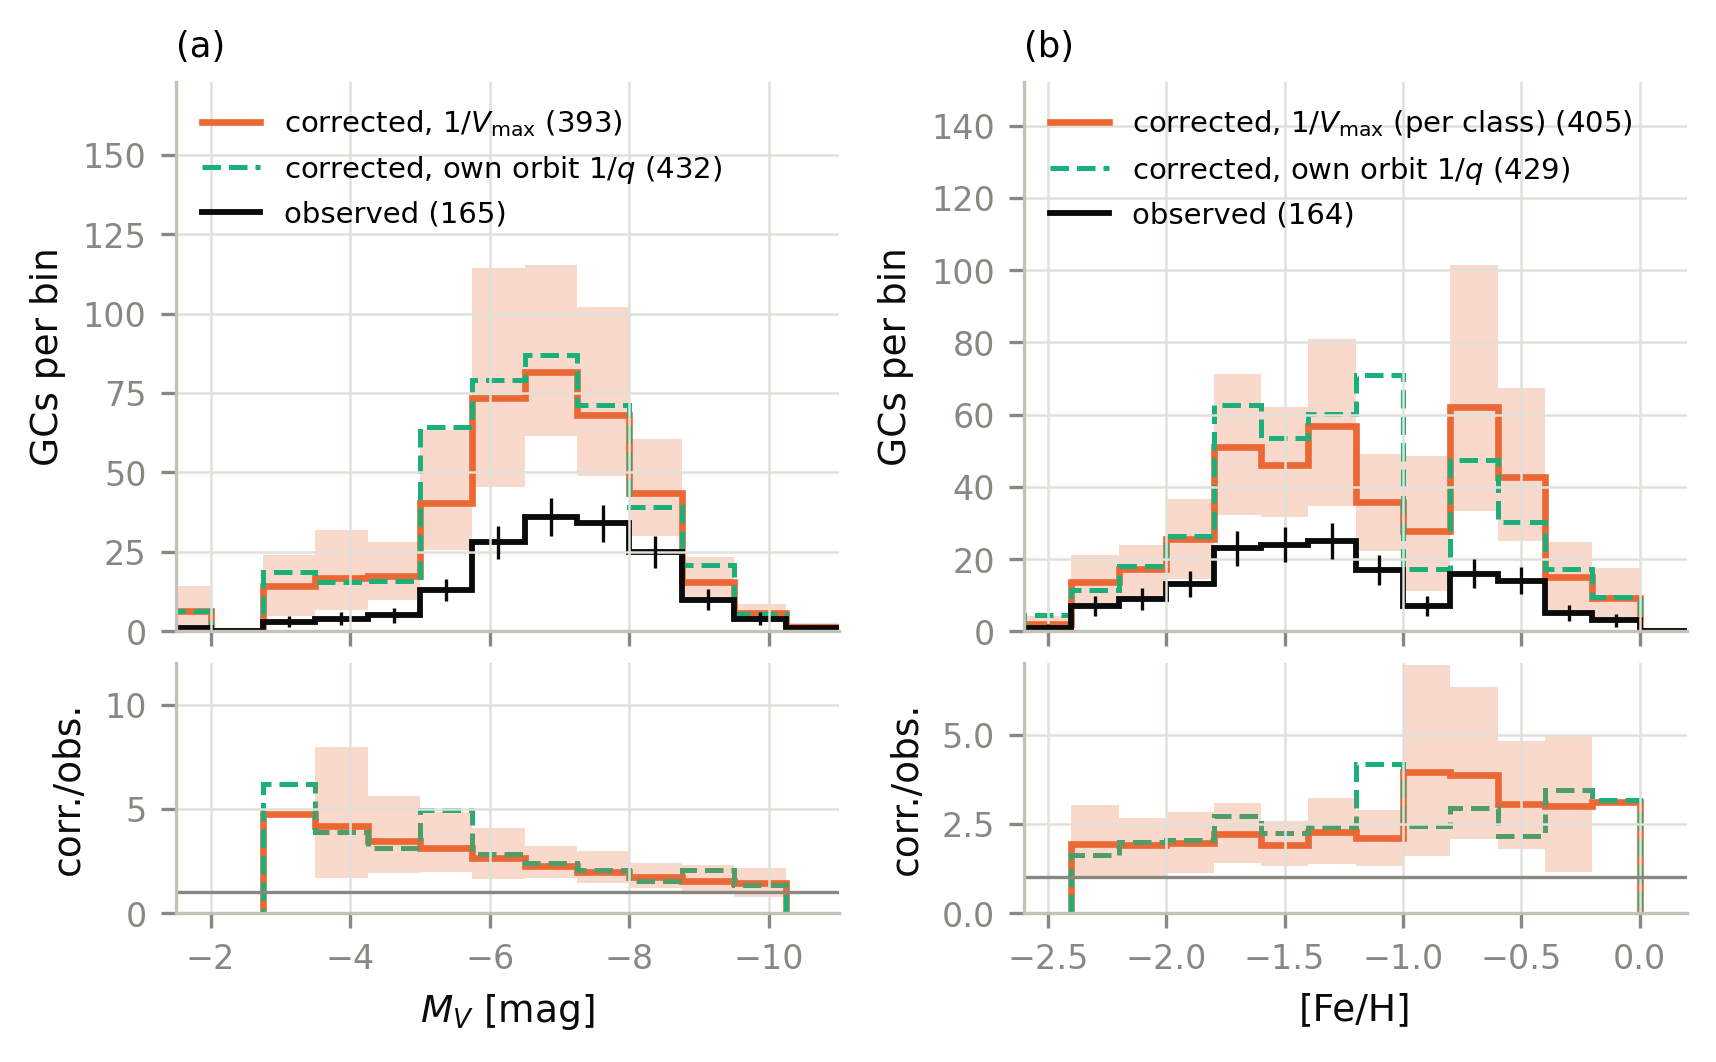
\includegraphics[width=\textwidth]{paper_corrected_vmax_map_high.png}
\caption{Corrected distributions with the continuous $C(V)$ and map extinction (high bracket):
$1/V_{\max}$ (solid; band: 68\% bootstrap) and own-orbit $1/q$ (dashed). (a) $\MV$, with the bright
clusters of all metallicities as orbit population. (b) [Fe/H], with $1/V_{\max}$ computed per class.}
\label{fig:vmax}
\end{figure}

\subsection{Which faint-end weighting? Realistic mocks and the shared-orbit assumption}
\label{sec:faint}

\paragraph{The question.} $1/V_{\max}$ assumes faint and bright GCs share one orbit distribution. If they
do, the detected faint clusters sit preferentially on the more detectable orbits, and the ratio
$R = $ faint$(1/V_{\max})/$faint$(1/q)$ exceeds 1: its median is 1.0--1.4 in the mocks of
Table~\ref{tab:vmax_mock}. On the real data $R = 0.85$ (maps) and 0.61 (no extinction): the observed
faint clusters lie on orbits \emph{less} detectable than those of bright clusters. If faint GCs are
preferentially on extended orbits, $1/V_{\max}$ undercounts them, and the mock-based preference for it
does not carry over. We therefore audited $R$, built mocks matched to the observed sample, and
compared four weightings on them, with acceptance tolerances fixed in advance (in
\texttt{configs/cv.yaml}): $|$median $\ln(N_{\rm corr}/N_{\rm true})| \le 0.10$ for totals and
$\le0.15$ for faint clusters, and 68\% coverage in $[0.59, 0.77]$. The four weightings are
\begin{itemize}
\item own-orbit $1/q$;
\item $1/V_{\max}$ with the bright clusters ($\MV<-8$) as orbit population;
\item a luminosity-matched $1/V_{\max}$, in which the population is all clusters weighted by
$1/q_j$ and by a Gaussian of width 1 mag in $\MV$;
\item $1/V_{\max}$ with the intermediate class ($-8\le\MV<-6.5$) as orbit population for faint targets.
\end{itemize}

\paragraph{Audit of $R$ on the real data.} With the maps (high bracket), $R = 0.85$ with a paired
bootstrap interval of $0.74$--$0.96$; it is below 1 in 92--94\% of resamples. Resampling the spline
node placement as well gives $0.73$--$0.96$. Three variants of the faint-end tail (an extra node at the
97.5th percentile of observed $V$, a flat tail, a tail twice as steep) and the per-[Fe/H] orbit
populations give $R = 0.77$--$0.89$; the low map bracket gives 0.79--0.89. The bright orbit population
is not dominated by a few clusters: its effective size is 31 of 40 and its largest normalised weight
8\%. So $R<1$ is not an artefact of the tail form or of a few weights.

\paragraph{Apocentres.} The raw median apocentres of faint and bright GCs are 10.3 and 9.0 kpc
($\Delta\ln r_{\rm apo} = 0.13$, bootstrap $-0.39$ to $0.59$). Weighted by $1/q$ they are 14.1 and 5.8 kpc
($\Delta\ln r_{\rm apo} = 0.89$, $-0.05$ to $1.34$; positive in 82\% of resamples). The weighting itself
favours extended orbits for faint clusters, so only mocks can say what these numbers imply. Neither
statistic sees orbit families with no detected member.

\paragraph{Realistic mocks.} Mocks with the logistic truth of Sec.~\ref{sec:mocks}, at the observed sample
size, detect only 2--11 faint clusters against 55 real ones, because their logistic $C(V)$ falls far more steeply than the fitted one.
The new mocks use as true completeness the continuous $C(V)$ fitted to the real data (maps, high
bracket), a Gaussian luminosity function with mean $-6.8$ and width 1.5 mag, and 252 clusters, which
gives 167 detected, 54 of them faint, in the null case. Luminosity is drawn first; each class (bright,
intermediate, faint) is then sampled from its own isotropic DF with break radius scaled by $1$,
$\sqrt{s}$ and $s$. $s=1$ is the null (orbits independent of $\MV$); $s=2$ and $s=4$ make faint GCs
progressively more extended. We add the dust disc of scenario E, and two misspecification controls:
the logistic $C(V)$ and the power-law tail. Each scenario has 100 calibration and 100 validation
realisations; the mock design was fixed after a smoke test that showed detection counts only.

\begin{table}[h]
\centering
\caption{Validation mocks: median $\ln(N_{\rm corr}/N_{\rm true})$ for the total and for faint clusters
($\MV\ge-6.5$), 100 realisations per scenario. Columns: own-orbit $1/q$; $1/V_{\max}$ with the bright
orbit population; luminosity-matched (kernel) $1/V_{\max}$; $1/V_{\max}$ with the intermediate class as
population for faint targets. Last two rows: misspecification controls.}
\label{tab:faint_mock}
\small\setlength{\tabcolsep}{4pt}
\begin{tabular}{lcccc}
\toprule
Scenario & $1/q$: total, faint & $1/V_{\max}$: total, faint & kernel: faint & intermediate: faint \\
\midrule
Null ($s=1$), real $C$ & $-0.06$, $-0.12$ & $-0.14$, $-0.16$ & $-0.12$ & $-0.13$ \\
Null + dust disc & $+0.05$, $+0.10$ & $+0.02$, $+0.01$ & $+0.09$ & $+0.04$ \\
$s=2$ & $+0.06$, $+0.07$ & $-0.08$, $-0.17$ & $+0.02$ & $-0.04$ \\
$s=4$ & $+0.13$, $+0.15$ & $-0.03$, $-0.14$ & $+0.09$ & $-0.02$ \\
$s=4$ + dust disc & $+0.12$, $+0.13$ & $+0.02$, $-0.01$ & $+0.10$ & $+0.05$ \\
\midrule
Null, logistic $C$ & $-0.13$, $-0.35$ & $-0.08$, $-0.16$ & $-0.31$ & $-0.19$ \\
Null, power-law tail & $+0.12$, $+0.15$ & $+0.00$, $-0.09$ & $+0.14$ & $-0.01$ \\
\bottomrule
\end{tabular}
\end{table}

\paragraph{Results (Table~\ref{tab:faint_mock}).}
\begin{itemize}
\item \textbf{The intervals are calibrated once the mocks resemble the data.} The 68\% bootstrap
intervals (node placement resampled) cover the truth in 63--79\% of validation realisations for every
weighting and scenario. The factor that would make them cover exactly 68\% on the calibration set is
0.92--1.03, so no inflation is needed. The 53--70\% coverage of Sec.~\ref{sec:vmax} came from the
small, steeply selected samples of the earlier mocks.
\item \textbf{No weighting is reliably better.} All four are within $\pm0.17$ in median $\ln$ in the
realistic scenarios, and the scatter of a single sample is large (rms $\ln$ 0.36--0.61 for totals,
0.44--0.74 for faint clusters). The standard error of each median bias is 0.04--0.07, comparable to
the differences between weightings, and on the same realisations the intermediate-class version
changes $|\ln|$ errors by at most 0.04 relative to the others, with 95\% intervals that include
zero in nearly every scenario. Its apparent advantage in the $s>1$ scenarios is also favoured by the
mock design, whose orbit trend changes at exactly its class boundaries. The bright-population
$1/V_{\max}$ is biased low even in the null ($-0.14$, $-0.16$).
\item \textbf{The misspecification controls fail for all weightings} at the faint end ($-0.16$ to
$-0.35$ for the logistic truth), as expected when $C(V)$ is poorly represented.
\end{itemize}

\paragraph{Do faint GCs have more extended orbits?} Table~\ref{tab:faint_diag} compares the real values
of $R$ and of the apocentre differences with their mock distributions. The real data fit a mild trend
($s=2$) best. A strong trend ($s=4$) is disfavoured: only 2--4\% of those mocks have a raw apocentre
difference as small as observed. No trend is not excluded: each statistic alone has a probability of
0.1--0.2 under the null, and $R$ and the weighted apocentre difference jointly 0.02--0.09.

\begin{table}[h]
\centering
\caption{Fraction of validation and calibration mocks (200 per scenario) at least as extreme as the real
data: $R\le0.85$; $1/q$-weighted $\Delta\ln r_{\rm apo}\ge0.89$; raw $\Delta\ln r_{\rm apo}\ge0.13$.}
\label{tab:faint_diag}
\small
\begin{tabular}{lccc}
\toprule
Scenario & $R\le0.85$ & weighted $\Delta\ln r_{\rm apo}\ge0.89$ & raw $\Delta\ln r_{\rm apo}\ge0.13$ \\
\midrule
Null ($s=1$) & 0.16 & 0.10 & 0.18 \\
Null + dust disc & 0.16 & 0.02 & 0.21 \\
$s=2$ & 0.40 & 0.30 & 0.79 \\
$s=4$ & 0.64 & 0.74 & 0.98 \\
$s=4$ + dust disc & 0.44 & 0.68 & 0.96 \\
\bottomrule
\end{tabular}
\end{table}

\paragraph{Choice.} We take own-orbit $1/q$ as the headline weighting: it needs no choice of orbit
population, passes in the null and mild-trend mocks, and is the closest to unbiased in the case the
data favour. The other three give the sensitivity range. With the continuous $C(V)$ and the maps
(high bracket) the corrected total is 432 ($321$--$628$) with $1/q$ and 393--432 across the four
weightings; faint clusters number 208 ($137$--$314$) and 177--208. The low map bracket raises all
values by 6--8\%.

\subsection{Direction-dependent completeness}
\label{sec:region}

\paragraph{Model.} Sec.~\ref{sec:nodustbias} shows that a single $C(V)$ can carry the selection of one
part of the sky into another. We therefore let completeness depend on direction: each orbit sample is
assigned to the inner window $|l|<30^\circ$, $|b|<15^\circ$ (fixed before fitting) or to the rest of
the sky, and $\ln C$ is evaluated with that region's curve. The rest of the sky carries the anchor. We
fit two forms: a shared continuous curve
plus a constant inner contrast (one extra parameter), and separate continuous curves per region, with
nodes at the median present $V$ of the clusters now in each region. The inner level is constrained by
orbits that cross between regions: 86 clusters spend 10--90\% of their orbit in each, while 39 stay
in the window throughout. Both weightings carry over unchanged, with every orbit sample using its
region's $C$.

\paragraph{Mocks.} We added three scenarios to those of Sec.~\ref{sec:mocks}, 100 realisations each:
H, a shallower limit inside the window ($V_{\rm lim}=6$ against 8 outside); I, a constant factor 0.5
inside the window; and J, a direction effect in a larger window ($|l|<60^\circ$, $|b|<25^\circ$) than
the one fitted. Table~\ref{tab:region_mock} gives the bias and scatter of the total.
\begin{itemize}
\item \textbf{The contrast model does no harm when there is no direction effect} (A, F, B, E, C: paired
ratio to the single curve 1.00--1.01), and the AIC prefers it falsely in 14--26\% of those mocks, close
to the 16\% expected for one extra parameter.
\item \textbf{It detects a direction effect inside the window} (AIC preference 98\% in H, 81\% in I) and
removes most of the bias (H: $-0.10$ to $+0.01$; I: $-0.16$ to $-0.05$).
\item \textbf{It does not fix a direction effect outside the fitted window} (J: $+0.17$).
\item \textbf{The separate curves have 30\% less scatter}, but a control fit shows this comes from their
fewer nodes per region: a single curve with as few nodes has the same scatter but is biased by $+0.2$
to $+0.4$ in H, J and E, where the separate curves are not.
\end{itemize}

\begin{table}[h]
\centering
\caption{Mocks with direction-dependent completeness: mean and rms of $\ln(N_{\rm corr}/N_{\rm true})$ for the
total ($1/q$), 100 realisations per scenario, and the fraction of mocks in which the AIC prefers the contrast
model over the single curve.}
\label{tab:region_mock}
\small\setlength{\tabcolsep}{4pt}
\begin{tabular}{lcccc}
\toprule
Scenario & Single $C(V)$ & Shared + contrast & Separate curves & AIC: contrast \\
\midrule
A: no direction effect & $-0.04$ / 0.51 & $-0.03$ / 0.51 & $+0.06$ / 0.35 & 15\% \\
F: two surveys & $+0.10$ / 0.51 & $+0.10$ / 0.51 & $+0.15$ / 0.36 & 15\% \\
H: shallower limit in window & $-0.10$ / 0.51 & $+0.01$ / 0.45 & $+0.03$ / 0.39 & 98\% \\
I: factor 0.5 in window & $-0.16$ / 0.48 & $-0.05$ / 0.44 & $+0.13$ / 0.37 & 81\% \\
J: effect outside fitted window & $+0.13$ / 0.50 & $+0.17$ / 0.51 & $+0.13$ / 0.44 & 44\% \\
B: latitude band & $-0.11$ / 0.50 & $-0.09$ / 0.49 & $-0.04$ / 0.34 & 26\% \\
E: dust disc & $-0.18$ / 0.45 & $-0.18$ / 0.44 & $+0.04$ / 0.35 & 14\% \\
\bottomrule
\end{tabular}
\end{table}

\paragraph{Real data} (Table~\ref{tab:region_real}, Fig.~\ref{fig:region}). We treat the regional
models as a test of how sensitive the result is to direction-dependent selection, not as a substitute
for the extinction maps.
\begin{itemize}
\item \textbf{Without extinction the data prefer direction dependence}: the separate curves are
preferred by $\Delta{\rm AIC}=-4.2$, with the inner curve falling well below the outer one at faint $V$
($\ln C_{\rm in}-\ln C_{\rm out}=-1.65$ at $V=12$). As expected from Sec.~\ref{sec:nodustbias}, the weights
of clusters now in the window rise (summed $1/q$: 186 to 299), and the total rises from 749 to 802.
\item \textbf{But the two-region split leaves most of the no-dust halo excess in place.} The summed $1/q$
of the 43 GCs at $\dhel>15$ kpc falls only from 453 to 376, against 135 with the maps, because the outer
curve stays steep ($C_{\rm out}=0.064$ at $V=14$ without dust, 0.23 with the maps). Although 84\% of
the orbit samples with $A_V>1$ lie inside the window, that steepness is not set by the halo clusters or by
dusty sightlines outside the window. Decomposing $\partial\ln L/\partial\lambda$, where $\lambda$ scales
the outer curve's $\ln C$, into per-cluster terms shows that the pull towards a steeper outer curve
comes from the 41 clusters now inside the window whose orbits leave it ($+10.3$, balanced by $-9.5$ from
the 77 now outside whose orbits enter it). The halo clusters ($-2.1$) and the clusters with dusty
off-window orbit segments ($-2.3$) pull the other way. The two regional curves are coupled through these
crossing orbits: the extra loss of inner clusters that the model cannot attribute to dust is partly
assigned to the outer curve, which then also applies to the halo. A third region (low latitude outside
the window, $|b|<15^\circ$) removes more of the excess (halo 257, total 575, $\Delta{\rm AIC}=-4.2$ against
two regions) but not all of it. No single cluster dominates: in leave-one-out refits the ten most
influential clusters carry 26\% of the total influence on the halo weight.
\item \textbf{With the 3D maps the data do not prefer extra direction dependence}: $\Delta{\rm AIC}=+1.0$
(contrast), $0.0$ (two separate curves) and $-1.1$ (three regions). The remaining inner/outer contrast of the
two-region fits is $\ln C_{\rm in}-\ln C_{\rm out}=-0.27$ ($-0.53$ to $-0.02$), a factor of about 0.76 at all
$V$.
\item \textbf{The totals move by $-12$ to $+12\%$} (432 to 380--485 with $1/q$, maps high): 453 and 485 with
two regions, 380 with three (halo weight 82). The intervals are no wider for the two-region models, with
$p_{84}/p_{16}$ 1.96--1.99 for all three. The three-region fit has only 19 clusters now in its
low-latitude region and two nodes there, so we do not adopt it.
\item A check of the model, the $C$-weighted version of the $u$ test above, passes inside the window
($p\approx0.6$) under every model, and fails mildly outside it ($p=0.01$--0.025) under every model, with
or without the maps. Neither a regional curve nor the maps account for that residual, so some mismatch
between model and data remains possible.
\end{itemize}

\begin{table}[h]
\centering
\caption{Real data: corrected totals with direction-dependent $C$; $\Delta{\rm AIC}$ relative to the single
continuous $C(V)$ with the same extinction; 68\% bootstrap intervals.}
\label{tab:region_real}
\small\setlength{\tabcolsep}{3pt}
\begin{tabular}{lcccccc}
\toprule
 & \multicolumn{3}{c}{No extinction} & \multicolumn{3}{c}{Maps, high bracket} \\
Model & $\Delta$AIC & $1/q$ & $1/V_{\max}$ & $\Delta$AIC & $1/q$ & $1/V_{\max}$ \\
\midrule
Single $C(V)$ & 0 & 749 ($467$--$1185$) & 563 ($348$--$841$) & 0 & 432 ($321$--$628$) & 393 ($274$--$573$) \\
Shared + contrast & $-0.9$ & 732 ($485$--$1261$) & 567 ($384$--$875$) & $+1.0$ & 453 ($333$--$657$) & 408 ($298$--$559$) \\
Separate curves & $-4.2$ & 802 ($592$--$1334$) & 671 ($491$--$938$) & $+0.0$ & 485 ($361$--$719$) & 437 ($316$--$598$) \\
\bottomrule
\end{tabular}
\end{table}

\begin{figure}[h]
\centering
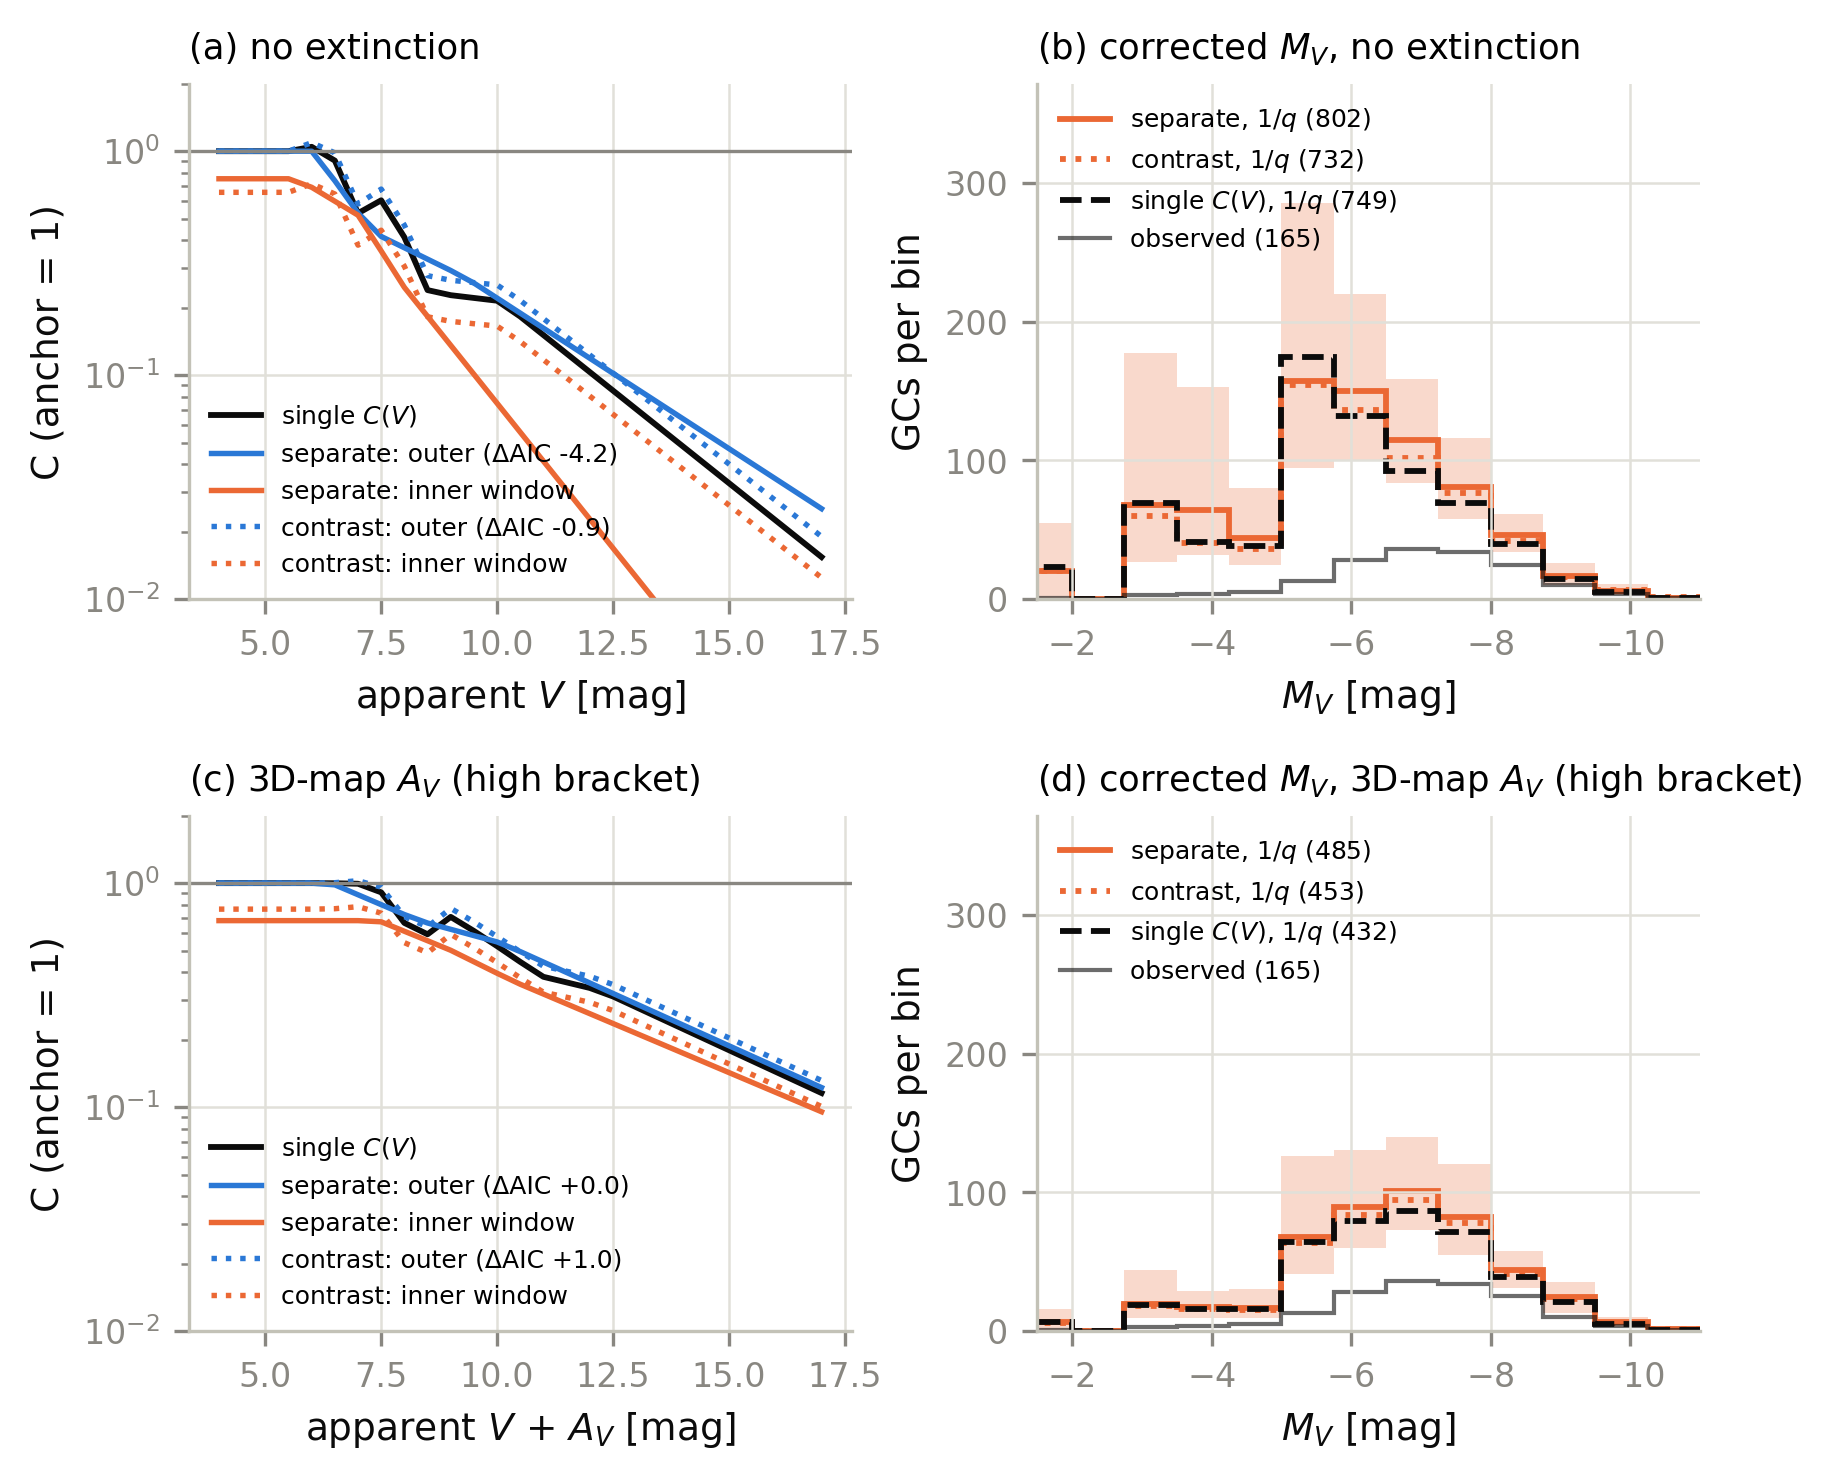
\includegraphics[width=\textwidth]{paper_region.png}
\caption{Direction-dependent completeness without extinction (top) and with map extinction (bottom, high
bracket). (a, c) $C$ for the single curve (black), and for the outer sky (blue) and the inner window
$|l|<30^\circ$, $|b|<15^\circ$ (orange), with separate curves (solid) or a shared curve plus a constant
contrast (dotted). (b, d) Corrected $\MV$ distributions with $1/q$; band: 68\% bootstrap for the separate
curves.}
\label{fig:region}
\end{figure}

%======================================================================
\section{Summary of results and error budget}
\label{sec:budget}

With continuous $C(V)$, 3D-map extinction (high bracket) and own-orbit weights, the 165 GCs with 6D
data correct to $432$ ($68\%$: $321$--$628$), about 2.6 times the observed number, of which $208$
($137$--$314$) are fainter than $\MV=-6.5$, against 55 observed. Table~\ref{tab:budget} lists how
each choice moves the total. The refinements of the weighting, the faint tail and the direction
dependence move it by up to 12\%; the bootstrap interval spans $-26$ to $+45\%$. The two changes that
matter are the extinction along the orbits, a factor of 1.7, and the continuous $C(V)$, which in mocks
fixed a factor-of-two undercount of faint clusters. The systematics in the last three rows are not yet
quantified.

\begin{table}[h]
\centering
\caption{Error budget for the corrected total (continuous $C(V)$, maps high bracket, $1/q$: 432).}
\label{tab:budget}
\small
\begin{tabular}{lll}
\toprule
Source & Range of the total & Relative \\
\midrule
Sampling (cluster bootstrap, 68\%) & 321--628 & $-26$\%, $+45$\% \\
Weighting ($1/q$, three $1/V_{\max}$ forms) & 393--432 & $-9$\% \\
Faint-end tail shape (three variants) & 424--457 & $-2$\%, $+6$\% \\
Direction-dependent $C$ (two or three regions) & 380--485 & $-12$\%, $+12$\% \\
Map bracket (high, low) & 432--461 & $+7$\% \\
Extinction treatment (none vs maps) & 749 vs 432--461 & factor 1.7 \\
Anchor (brightest $V$ complete) & all weights scale as $1/C_{\rm anchor}$ & not quantified \\
Phase mixing, static potential, orbit errors & --- & not quantified \\
Clusters on never-detectable orbits & --- & not identifiable \\
\bottomrule
\end{tabular}
\end{table}

\subsection{The final answer}
\label{sec:final}

\begin{equation}
N_{\rm GC} \approx 430^{+215}_{-125}\qquad(68\%,\ \text{sampling and quantified systematics}),
\label{eq:final}
\end{equation}
about 2.6 times the 165 GCs with 6D data. Of these, about 210 (68\%: 125--325, sampling and quantified systematics; 140--315 from sampling alone) are
fainter than $\MV=-6.5$, against 55 observed (Fig.~\ref{fig:final}).

\begin{figure}[h]
\centering
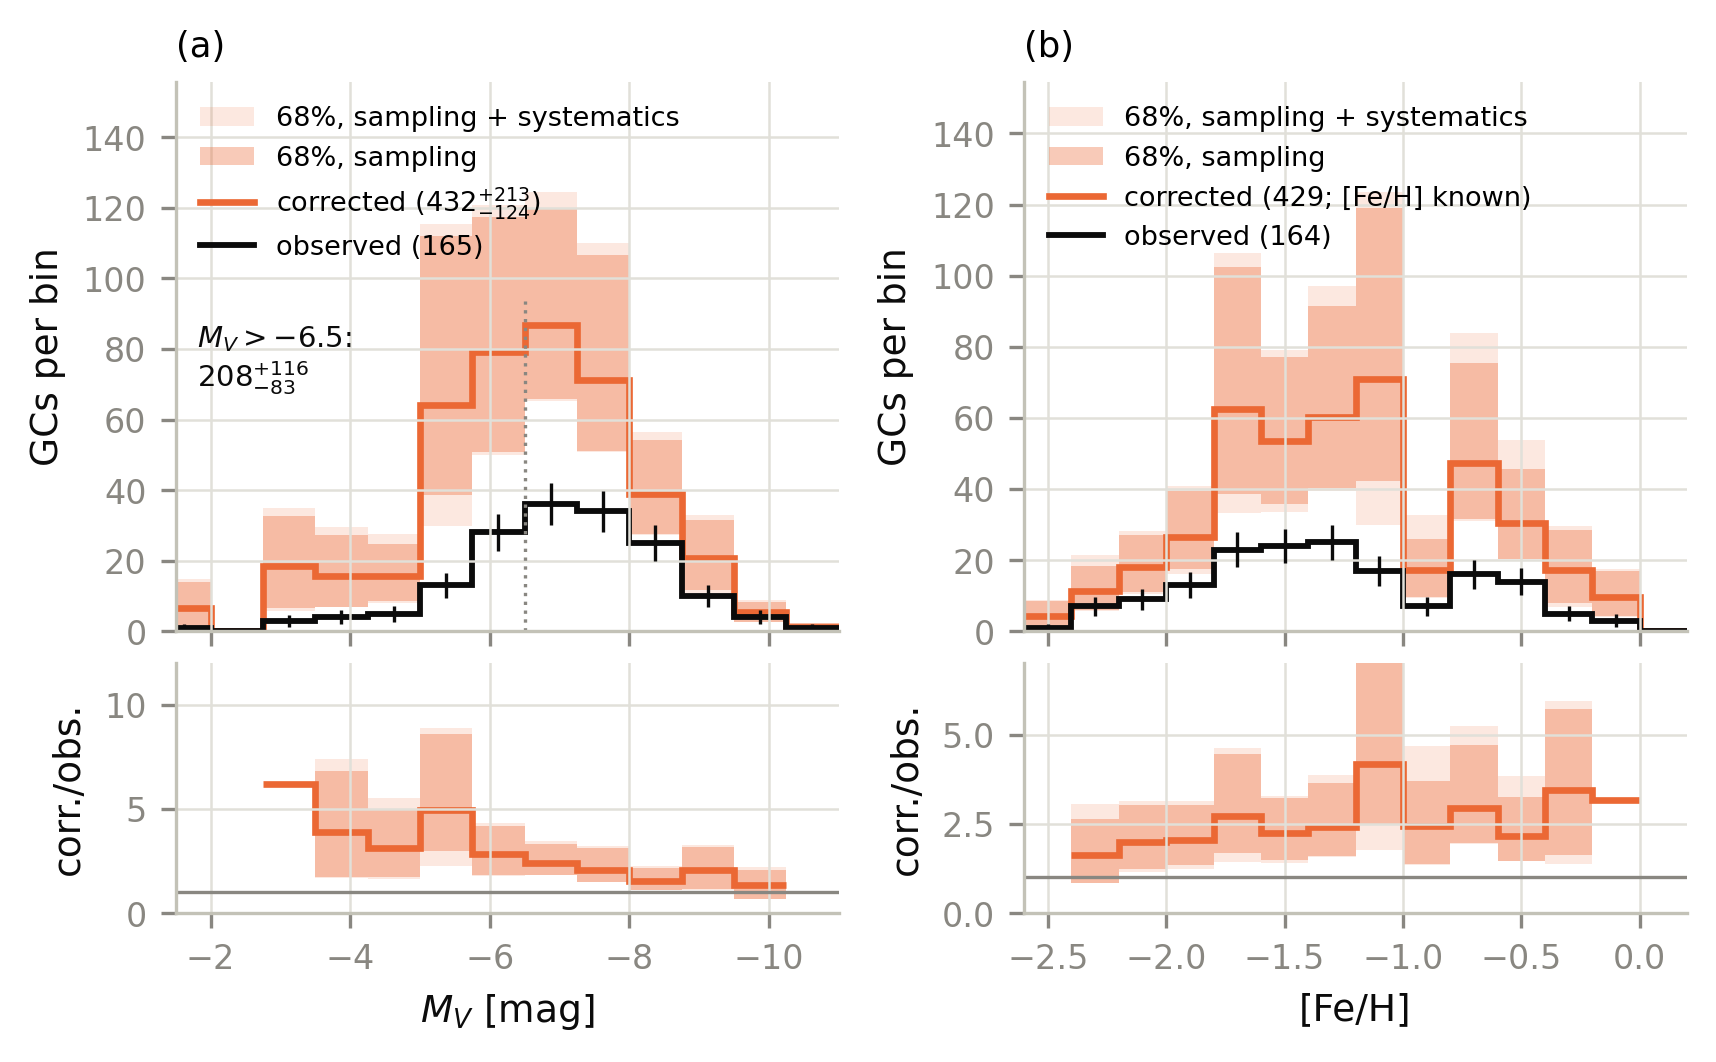
\includegraphics[width=\textwidth]{paper_final.png}
\caption{The final model: corrected $\MV$ (a) and [Fe/H] (b) distributions with the continuous $C(V)$,
3D-map extinction (high bracket) and own-orbit $1/q$ weights. Dark band: 68\% cluster bootstrap
(sampling); light band: sampling and the quantified systematics in quadrature. The systematic part is
evaluated in each bin from the per-cluster weights of every alternative in Table~\ref{tab:budget} (weighting,
tail shape, direction-dependent $C$, map bracket): for each component, the largest downward and upward
change of the bin count, then quadrature over components. The legend in (a) gives the total and the faint
count with the same construction (Eq.~\ref{eq:final}); (b) omits the one cluster without [Fe/H]. Lower
panels: corrected/observed. The bootstrap band is calibrated in mocks for the total and faint counts only;
in bins with a few observed clusters it is coarse.}
\label{fig:final}
\end{figure}

\paragraph{What the central value is.} The total from the continuous $C(V)$ (Sec.~\ref{sec:vmax}), with
extinction from 3D maps along every orbit (high bracket, Sec.~\ref{sec:ext}) and each cluster weighted by
the inverse of its own orbit-averaged completeness, $1/q_i$: 432. This is the model the likelihood prefers
(Table~\ref{tab:vmax_real}); ignoring extinction (749) is rejected by $\Delta{\rm AIC}\approx16$ and biased
high for the reason given in Sec.~\ref{sec:nodustbias}.

\paragraph{How the error bar is built.} We work in $\ln N$ and take each component's largest excursion
from Table~\ref{tab:budget}:
\begin{center}
\small
\begin{tabular}{lcc}
\toprule
Component & down & up \\
\midrule
Sampling (cluster bootstrap, 321--628) & $-0.30$ & $+0.37$ \\
Weighting (393--432) & $-0.10$ & 0 \\
Faint-tail shape (424--457) & $-0.02$ & $+0.06$ \\
Direction-dependent $C$ (380--485) & $-0.13$ & $+0.12$ \\
Map bracket (432--461) & 0 & $+0.07$ \\
\midrule
Quantified systematics, in quadrature & $-0.16$ & $+0.14$ \\
Total, in quadrature & $-0.34$ & $+0.40$ \\
\bottomrule
\end{tabular}
\end{center}
The total gives factors of $e^{-0.34}=0.71$ and $e^{0.40}=1.49$, i.e.\ 308--645 around 432. The sampling
part is calibrated: in mocks matched to the observed sample, the 68\% bootstrap intervals cover the truth in
63--79\% of realisations (Sec.~\ref{sec:faint}). The systematic ranges are spreads between model choices,
not Gaussian errors. Adding the systematic total linearly to the sampling error instead ($-0.46$, $+0.52$)
gives 275--725; adding every component linearly ($-0.54$, $+0.61$) gives 250--795. For the faint count the same construction gives systematics of $-0.29$ and $+0.16$, larger than
for the total: the three-region $C$ ($-0.24$) and the $1/V_{\max}$ weighting ($-0.16$) both lower it, so
the faint count is $208^{+116}_{-83}$ (125--325).

\paragraph{What is not in the error bar.} Three effects are not quantified. If the brightest clusters,
which anchor $C$, are themselves incomplete, every weight rises; clusters on orbits that are never
detectable are counted by none of our weightings. Both can only increase $N$. Errors in the Galactic
potential, the orbits and the phase-mixing assumption have unknown sign. Equation~\ref{eq:final} is
therefore best read as about 430, most likely between 310 and 650, with the unquantified effects pointing
upwards.

%======================================================================
\section{Limitations and next steps}
\label{sec:limits}

\begin{enumerate}
\item \textbf{Unseen orbit families.} No weighting counts orbit families with no detected member
unless an orbit population is assumed. The data favour at most a mild trend of orbit size with
luminosity (Sec.~\ref{sec:faint}); a stronger one would make all four weightings low for faint clusters.
\item \textbf{Extinction.} The 3D-map treatment rests on fixed conversions (in particular
$A_V = 8.8\,A_{K_s}$ for Marshall, uncertain in the inner Galaxy) and on SFD beyond the maps' reach.
Map uncertainties and alternative extinction laws are not propagated beyond the low/high brackets;
mocks with map-based rather than analytic dust would test the full chain.
\item \textbf{Anchor.} All absolute numbers assume the brightest-$V$ clusters are complete. Every weight
scales as $1/C_{\rm anchor}$; an independent census of the brightest GCs would test it.
\item \textbf{Potential, phase mixing and orbit errors.} The intervals cover sampling noise only. An
ensemble of perturbed phase-space coordinates and alternative potentials would give the systematic
spread. The $u$ test fails mildly for clusters outside the inner window ($p=0.01$--0.025) under every
completeness model (Sec.~\ref{sec:region}); groups that are not phase-mixed, such as the clusters of
the Sagittarius dwarf, which all sit near the inner parts of their orbits, are one candidate.
\item \textbf{Mock realism.} The calibrated coverage of Sec.~\ref{sec:faint} holds for mocks whose true
completeness is the fitted one and whose population is quasi-spherical and isotropic; the misspecified
controls show biases of up to $-0.35$ in $\ln$ for faint clusters.
\end{enumerate}

%======================================================================
\begin{thebibliography}{9}
\bibitem{astropy22} Astropy Collaboration et al.\ 2022, ApJ, 935, 167,
\href{https://doi.org/10.3847/1538-4357/ac7c74}{doi:10.3847/1538-4357/ac7c74}
\bibitem{green19} Green G.~M.\ et al.\ 2019, ApJ, 887, 93,
\href{https://doi.org/10.3847/1538-4357/ab5362}{doi:10.3847/1538-4357/ab5362}
\bibitem{ht52} Horvitz D.~G., Thompson D.~J.\ 1952, J.\ Am.\ Stat.\ Assoc., 47, 663,
\href{https://doi.org/10.1080/01621459.1952.10483446}{doi:10.1080/01621459.1952.10483446}
\bibitem{khop25} Khoperskov S.\ et al.\ 2025, A\&A, 695, A220,
\href{https://doi.org/10.1051/0004-6361/202453304}{doi:10.1051/0004-6361/202453304},
\href{https://arxiv.org/abs/2411.15062}{arXiv:2411.15062}
\bibitem{marshall06} Marshall D.~J.\ et al.\ 2006, A\&A, 453, 635,
\href{https://doi.org/10.1051/0004-6361:20053842}{doi:10.1051/0004-6361:20053842}
\bibitem{massari19} Massari D., Koppelman H.~H., Helmi A.\ 2019, A\&A, 630, L4,
\href{https://doi.org/10.1051/0004-6361/201936135}{doi:10.1051/0004-6361/201936135}
\bibitem{sf11} Schlafly E.~F., Finkbeiner D.~P.\ 2011, ApJ, 737, 103,
\href{https://doi.org/10.1088/0004-637X/737/2/103}{doi:10.1088/0004-637X/737/2/103}
\bibitem{sfd98} Schlegel D.~J., Finkbeiner D.~P., Davis M.\ 1998, ApJ, 500, 525,
\href{https://doi.org/10.1086/305772}{doi:10.1086/305772}
\bibitem{schmidt68} Schmidt M.\ 1968, ApJ, 151, 393,
\href{https://doi.org/10.1086/149446}{doi:10.1086/149446}
\bibitem{vasiliev19} Vasiliev E.\ 2019, MNRAS, 482, 1525,
\href{https://doi.org/10.1093/mnras/sty2672}{doi:10.1093/mnras/sty2672}
\bibitem{vb21} Vasiliev E., Baumgardt H.\ 2021, MNRAS, 505, 5978,
\href{https://doi.org/10.1093/mnras/stab1475}{doi:10.1093/mnras/stab1475}
\bibitem{zucker25} Zucker C.\ et al.\ 2025, A deep, high-angular resolution 3D dust map of the southern
Galactic plane, \href{https://arxiv.org/abs/2503.02657}{arXiv:2503.02657}
\end{thebibliography}

\end{document}
